% !TeX root = Chapter_08_Risk_Finance_ART.tex
% Chapter 8 — Risk Finance and Alternative Risk Transfer
\documentclass[11pt,openany]{book}
\usepackage{graphicx}
\usepackage{amsmath,amssymb}
\usepackage{hanging}
\makeatletter
\def\input@path{{second_ed/style/}{../style/}}
\makeatother
\usepackage{erm_textbook_style}
\graphicspath{{second_ed/rscripts/chapter8/}{../rscripts/chapter8/}}
\providecommand{\tightlist}{\setlength{\itemsep}{0pt}\setlength{\parskip}{0pt}}
\emergencystretch=2em

\begin{document}

\setcounter{chapter}{7}
\chapter{Risk Finance and Alternative Risk Transfer}
\label{chap:risk-finance}

% -----------------------------------------------------------------------
\begin{learningobjectives}
  \item Explain the risk financing spectrum from full retention through
        traditional insurance to alternative risk transfer instruments, and
        identify where different strategies lie on the cost--volatility
        tradeoff curve.
  \item Calculate total cost of risk (TCOR) for retention versus transfer
        alternatives, incorporating expected losses, insurance expense loads,
        opportunity costs of capital, and administrative expenses.
  \item Design retention programs using deductibles and self-insured
        retentions (SIRs) that reduce TCOR while respecting the firm's risk
        appetite constraints.
  \item Evaluate the strategic and economic rationale for captive insurance
        companies, including structure, domicile, and tax considerations.
  \item Assess alternative risk transfer (ART) products including finite risk
        reinsurance, multi-trigger policies, integrated risk programs, and
        risk retention groups.
  \item Analyze catastrophe bonds and insurance-linked securities (ILS),
        including trigger design, basis risk, and the conditions under which
        capital market risk transfer beats traditional reinsurance.
  \item Integrate risk financing decisions with risk appetite
        (Chapter~5), portfolio analysis
        (Chapter~6), and loss control investments
        (Chapter~7).
\end{learningobjectives}

% -----------------------------------------------------------------------
\chapteroverview{%
After identifying risks, quantifying them, setting appetite boundaries,
aggregating them into an enterprise portfolio, and investing in loss control,
an organization faces the question that remains: \emph{who pays for the losses
that still occur?} Risk financing---the deliberate choice of who bears the
financial consequences of adverse events, and when---completes the ERM cycle
by converting everything the preceding chapters built into capital allocation
decisions.

This chapter maps the full menu of risk financing alternatives, from pure
retention (absorbing every loss internally) to complete transfer (insurance
and capital market instruments that shift risk to third parties). We examine
traditional insurance, self-insurance, captive insurance companies, and
alternative risk transfer mechanisms including catastrophe bonds and other
insurance-linked securities. The analytical thread running through the chapter
is total cost of risk (TCOR): every financing structure can be priced,
compared, and optimized against the firm's risk appetite. The opening
case---a theme park operator whose earthquake bond paid \textyen 10 billion
within weeks of the largest earthquake in Japanese history---shows where the
chapter is headed: risk financing at its best is not an insurance purchase
made out of habit, but an engineered answer to a quantified exposure.%
}

\clearpage

% -----------------------------------------------------------------------
% Opening Corporate Example: Oriental Land Company / Midori cat bond
% -----------------------------------------------------------------------
\begin{corporateexample}[The Bond That Paid When the Earth Moved]

The afternoon of March 11, 2011 began like most Fridays at the Tokyo
Disneyland Resort---crowds moving through the gates toward Cinderella Castle,
families queuing for rides, gift shops full. Oriental Land Company (OLC)\index{Oriental Land Company}, the
Japanese firm that licenses and operates the park, had just reported another
strong year. Attendance had climbed steadily since the park's 1983 opening.
The balance sheet was sound. And five years earlier, OLC's treasury team had
done something that most of its neighbors in the Tokyo Bay area had never
considered: they had sold a catastrophe bond.

OLC is not a household name outside Japan, but it operates one of the most
visited theme parks on earth. In a normal year, Tokyo Disneyland\index{Tokyo Disneyland} and its
sister park, Tokyo DisneySea, draw roughly 25 to 30 million guests. The
business model depends on continuous operations and an iconic physical
plant---hotels, rides, infrastructure, utilities---all concentrated on a
narrow strip of reclaimed land in Urayasu, Chiba Prefecture, directly on the
shoreline of Tokyo Bay. That geography, and the liquefaction risk that comes
with it, had long been visible to engineers and seismologists. The ground
beneath the resort was landfill, young and water-saturated, the kind of soil
that behaves like a liquid when shaken hard enough. OLC's risk managers knew
this. It sat in their catastrophe models, drove their engineering reviews, and
ultimately shaped a decision about where to look for protection.

In 2006, OLC completed a \textyen 10 billion catastrophe bond\index{Midori cat bond}\index{catastrophe bond} through a
special purpose vehicle called Midori Ltd. Investors worldwide purchased notes
issued by Midori, and the proceeds were held in a collateral trust. If a
qualifying earthquake struck a defined region of Japan at sufficient intensity
within the bond's term, the collateral would flow to OLC; if no trigger event
occurred, investors received their principal back along with premium coupons
that compensated them for bearing the risk. It was not insurance in the
conventional sense. There was no claims adjuster, no loss inspection, no
negotiation. The bond's trigger was parametric\index{parametric trigger}---it depended entirely on what
seismographs recorded at specified monitoring stations near the park. OLC had
gone to the capital markets to pre-arrange financing for a catastrophe it
hoped would never come.

At 2:46~p.m.\ on March 11, 2011, a magnitude 9.0 earthquake struck off the
Pacific coast of T\=ohoku---the largest earthquake ever recorded in Japan. The
ground motion radiated across Honshu in long, rolling waves. At Tokyo
Disneyland, the shaking lasted several minutes. Cast members guided guests
away from structures and onto open plazas, moving calmly through a script they
had rehearsed but never used at this scale. The park closed immediately. In
the hours that followed, as news from T\=ohoku arrived---the tsunami
overwhelming entire coastal towns, the reactor emergency at Fukushima---OLC's
damage assessment teams moved through both parks in the fading afternoon
light. The structures had held. The problem was the ground. Liquefaction had
materialized across large sections of the resort---pavements buckled and
cracked, utility lines ruptured, sections of the park simply sinking and
tilting as the saturated fill beneath them lost cohesion. The damage was
neither dramatic nor photogenic, but it was pervasive. Both parks went dark.

The operational response moved quickly. Within days, management had mobilized
contractors, and a repair effort that would eventually cost billions of yen
was underway. Workers pumped grout into the ground, re-leveled walkways,
replaced burst pipes, and worked in shifts to make the parks functional. Tokyo
Disneyland reopened in late March, DisneySea shortly after, faster than most
outside observers had expected.

The financial response moved through channels the guests never saw. OLC's
risk team and its advisers began evaluating the Midori bond against the
seismic data flowing in from the Japan Meteorological Agency's dense
monitoring network. The readings at the contractually specified measurement
points were reviewed against the trigger thresholds. The numbers were
unambiguous. The bond had triggered.

The collateral was released. Approximately \textyen 10 billion arrived---not
from an insurer's claims department, not through a reinsurance settlement that
might take months to negotiate, but through a capital market instrument that
settled like a bond because it was one. For the institutional investors who
had purchased the notes, the loss was real and final: principal was gone,
absorbed into OLC's reconstruction budget. For OLC, the payment was neither
luck nor windfall. It was the deliberate result of a decision made in 2006,
when the management team had looked at reclaimed land, at seismic maps, at
reinsurance pricing, and at a capital market that was willing to bear Japanese
earthquake risk at a price that made sense---and had structured a transaction
accordingly.

The repair work finished. The parks filled again. The Midori bond matured into
history, a line item in deal databases and a footnote in catastrophe bond
market retrospectives. In Urayasu, the ground was eventually stabilized
through a city-wide improvement program. The guests who returned in April 2011
walked over newly poured concrete and freshly painted surfaces, with no
particular reason to know that beneath the cheerful normalcy, a financial
instrument had performed exactly as its designers intended---quietly,
automatically, and on time.

\source{Artemis.bm cat bond database; OLC Annual Reports 2006--2012; Japan
Meteorological Agency seismic records; Guy Carpenter earthquake research.}
\end{corporateexample}

% =======================================================================
\section{Risk Financing Follows Risk Control}
\label{sec:financing-follows-control}

\subsection{The ERM Sequence: From Identification to Financing}

Enterprise risk management follows a logical progression. Chapters~3
through~6 focused on understanding risk: identifying hazard, financial,
operational, and strategic exposures; quantifying their frequency and severity
distributions; aggregating individual risks into portfolios; and comparing
total risk to organizational risk appetite. Chapter~7
examined loss control---systematic efforts to reduce loss frequency and
severity through engineering, administrative, and behavioral interventions.
Loss control is the first-order risk response: prevent losses from occurring,
or limit their magnitude when they do.

Risk financing\index{risk financing} addresses what remains. No organization can eliminate all
risk; some residual exposure persists because further loss control costs more
than it saves, because some hazards cannot be engineered away, or because the
organization must accept certain risks to pursue profitable opportunities.
Crestline Mutual's device program in Chapter~7 cut
electrical-fire losses sharply, but it did not cut them to zero---and nothing
Crestline could install in a policyholder's basement would address an
earthquake. Risk financing answers the question loss control leaves open:
\emph{given that losses will occur despite our best prevention efforts, how
should we pay for them?}

The distinction between risk control and risk financing is fundamental but
sometimes blurred in practice. Risk control modifies the underlying frequency
and severity of losses---the loss distribution itself shifts. Risk financing
does not change the distribution; it determines who bears the financial
consequences and when the cash flows occur. Installing sprinkler systems
(risk control) reduces both the probability of fires and the severity of
damage when fires occur. Purchasing property insurance (risk financing)
leaves fire frequency and severity exactly where they were but shifts the
financial burden from the organization to the insurer. OLC's catastrophe bond
did not make the ground beneath Tokyo Disneyland any firmer; it made sure
that when the ground failed, money arrived.

\subsection{The Risk Financing Decision Framework}

Risk financing decisions occur at three levels.

\textbf{Strategic level.} What proportion of enterprise-wide risk should we
retain versus transfer? This high-level decision reflects organizational risk
philosophy, financial capacity, and competitive strategy. Financially strong
organizations with diversified risk portfolios may deliberately retain more
risk to save on insurance transaction costs. Smaller or financially
constrained organizations may transfer more to preserve scarce capital for
operating investments.

\textbf{Portfolio level.} How should the risk financing budget be allocated
across risk categories---property, liability, workers' compensation, cyber?
The portfolio results of Chapter~6 matter here:
retaining uncorrelated risks provides natural diversification, while highly
correlated risks may warrant transfer to avoid concentration.

\textbf{Individual risk level.} For each specific exposure, should we retain
in full, transfer in full, or use hybrid structures (deductibles,
co-insurance, caps)? This tactical decision depends on loss characteristics
(frequency, severity, predictability), available market capacity, and
pricing.

These decisions interact. A strategic commitment to high retention requires
infrastructure---cash reserves, claims management capability, perhaps a
captive insurance entity---that creates economies of scale for retaining
individual risks. A strategic preference for transfer prevents that
infrastructure from developing, reinforcing dependence on external insurance
markets. Organizations rarely move along the spectrum quickly; the position
they occupy today usually reflects investments (or their absence) made years
earlier.

\subsection{Risk Financing and Organizational Value Creation}
\label{subsec:value-channels}

Recall from Chapter~1 that in a
frictionless Modigliani--Miller world\index{Modigliani-Miller theorem}, risk financing would be irrelevant:
shareholders could diversify on their own account, and paying an insurer's
expense load would destroy value. Risk financing creates value only through
the frictions that make the MM assumptions fail, and it pays to be specific
about which friction each channel exploits.

\textbf{Channel 1: Cost minimization.} Insurance premiums include expense
loads\index{expense load}---commissions, overhead, insurer profit---that typically add 25--40\%
to expected losses. Retaining predictable, high-frequency risks and
transferring only volatile, low-frequency exposures minimizes these
transaction costs (Harrington \& Niehaus, 2004).

\textbf{Channel 2: Cash flow timing.} Retention delays cash outflows until
losses occur, allowing investment of funds that would otherwise pay premiums
up front. For organizations with strong cash positions and investment
opportunities exceeding the risk-free rate, the timing advantage creates
value. Insurance does the reverse: it buys budgetary certainty at the cost of
accelerated outflows.

\textbf{Channel 3: Tax efficiency.} Tax treatment varies by mechanism.
Insurance premiums are immediately deductible (26 U.S.C. \S~162(a)), while
self-insured losses may be deductible only when paid or incurred. Captive
arrangements offer planning opportunities through premium deductibility and
domicile selection, though subject to anti-abuse rules (26 U.S.C.
\S\S~831(b), 482). Section~\ref{subsec:captive-tax} develops these issues.

\textbf{Channel 4: Reduced financial distress costs.}\index{financial distress} Transferring tail risk
through insurance or capital market instruments reduces the probability of
financial distress, bankruptcy, or covenant violations. This protection is
most valuable for firms with high leverage or thin liquidity (Froot,
Scharfstein, \& Stein, 1993). The OLC bond is exactly this channel at work:
pre-arranged contingent capital that arrives when internal resources are
under maximum strain.

\textbf{Channel 5: Managerial focus.} Executives spending months managing an
uninsured loss crisis are not running the business. Appropriate risk transfer
purchases management attention at reasonable cost. The channel is hard to
quantify and easy to overstate, but anyone who has watched a leadership team
improvise catastrophe financing under deadline pressure will not dismiss it.

The optimal strategy maximizes the sum of these value channels subject to
risk appetite constraints and available market capacity.
Sections~\ref{sec:retention-transfer} and~\ref{sec:tcor} develop the
analytical machinery.

% =======================================================================
\section{The Risk Financing Spectrum}
\label{sec:spectrum}

\subsection{The Continuum from Retention to Transfer}

Risk financing alternatives lie on a continuum\index{risk financing!spectrum} characterized by two
dimensions: \textbf{explicit cost} and \textbf{volatility reduction}.
Figure~\ref{fig:spectrum} illustrates the fundamental tradeoff: each step
from pure retention toward full transfer raises the explicit cost of
financing (premiums, fees, capital charges) and lowers the volatility the
organization retains.

\begin{figure}[htbp]
  \centering
  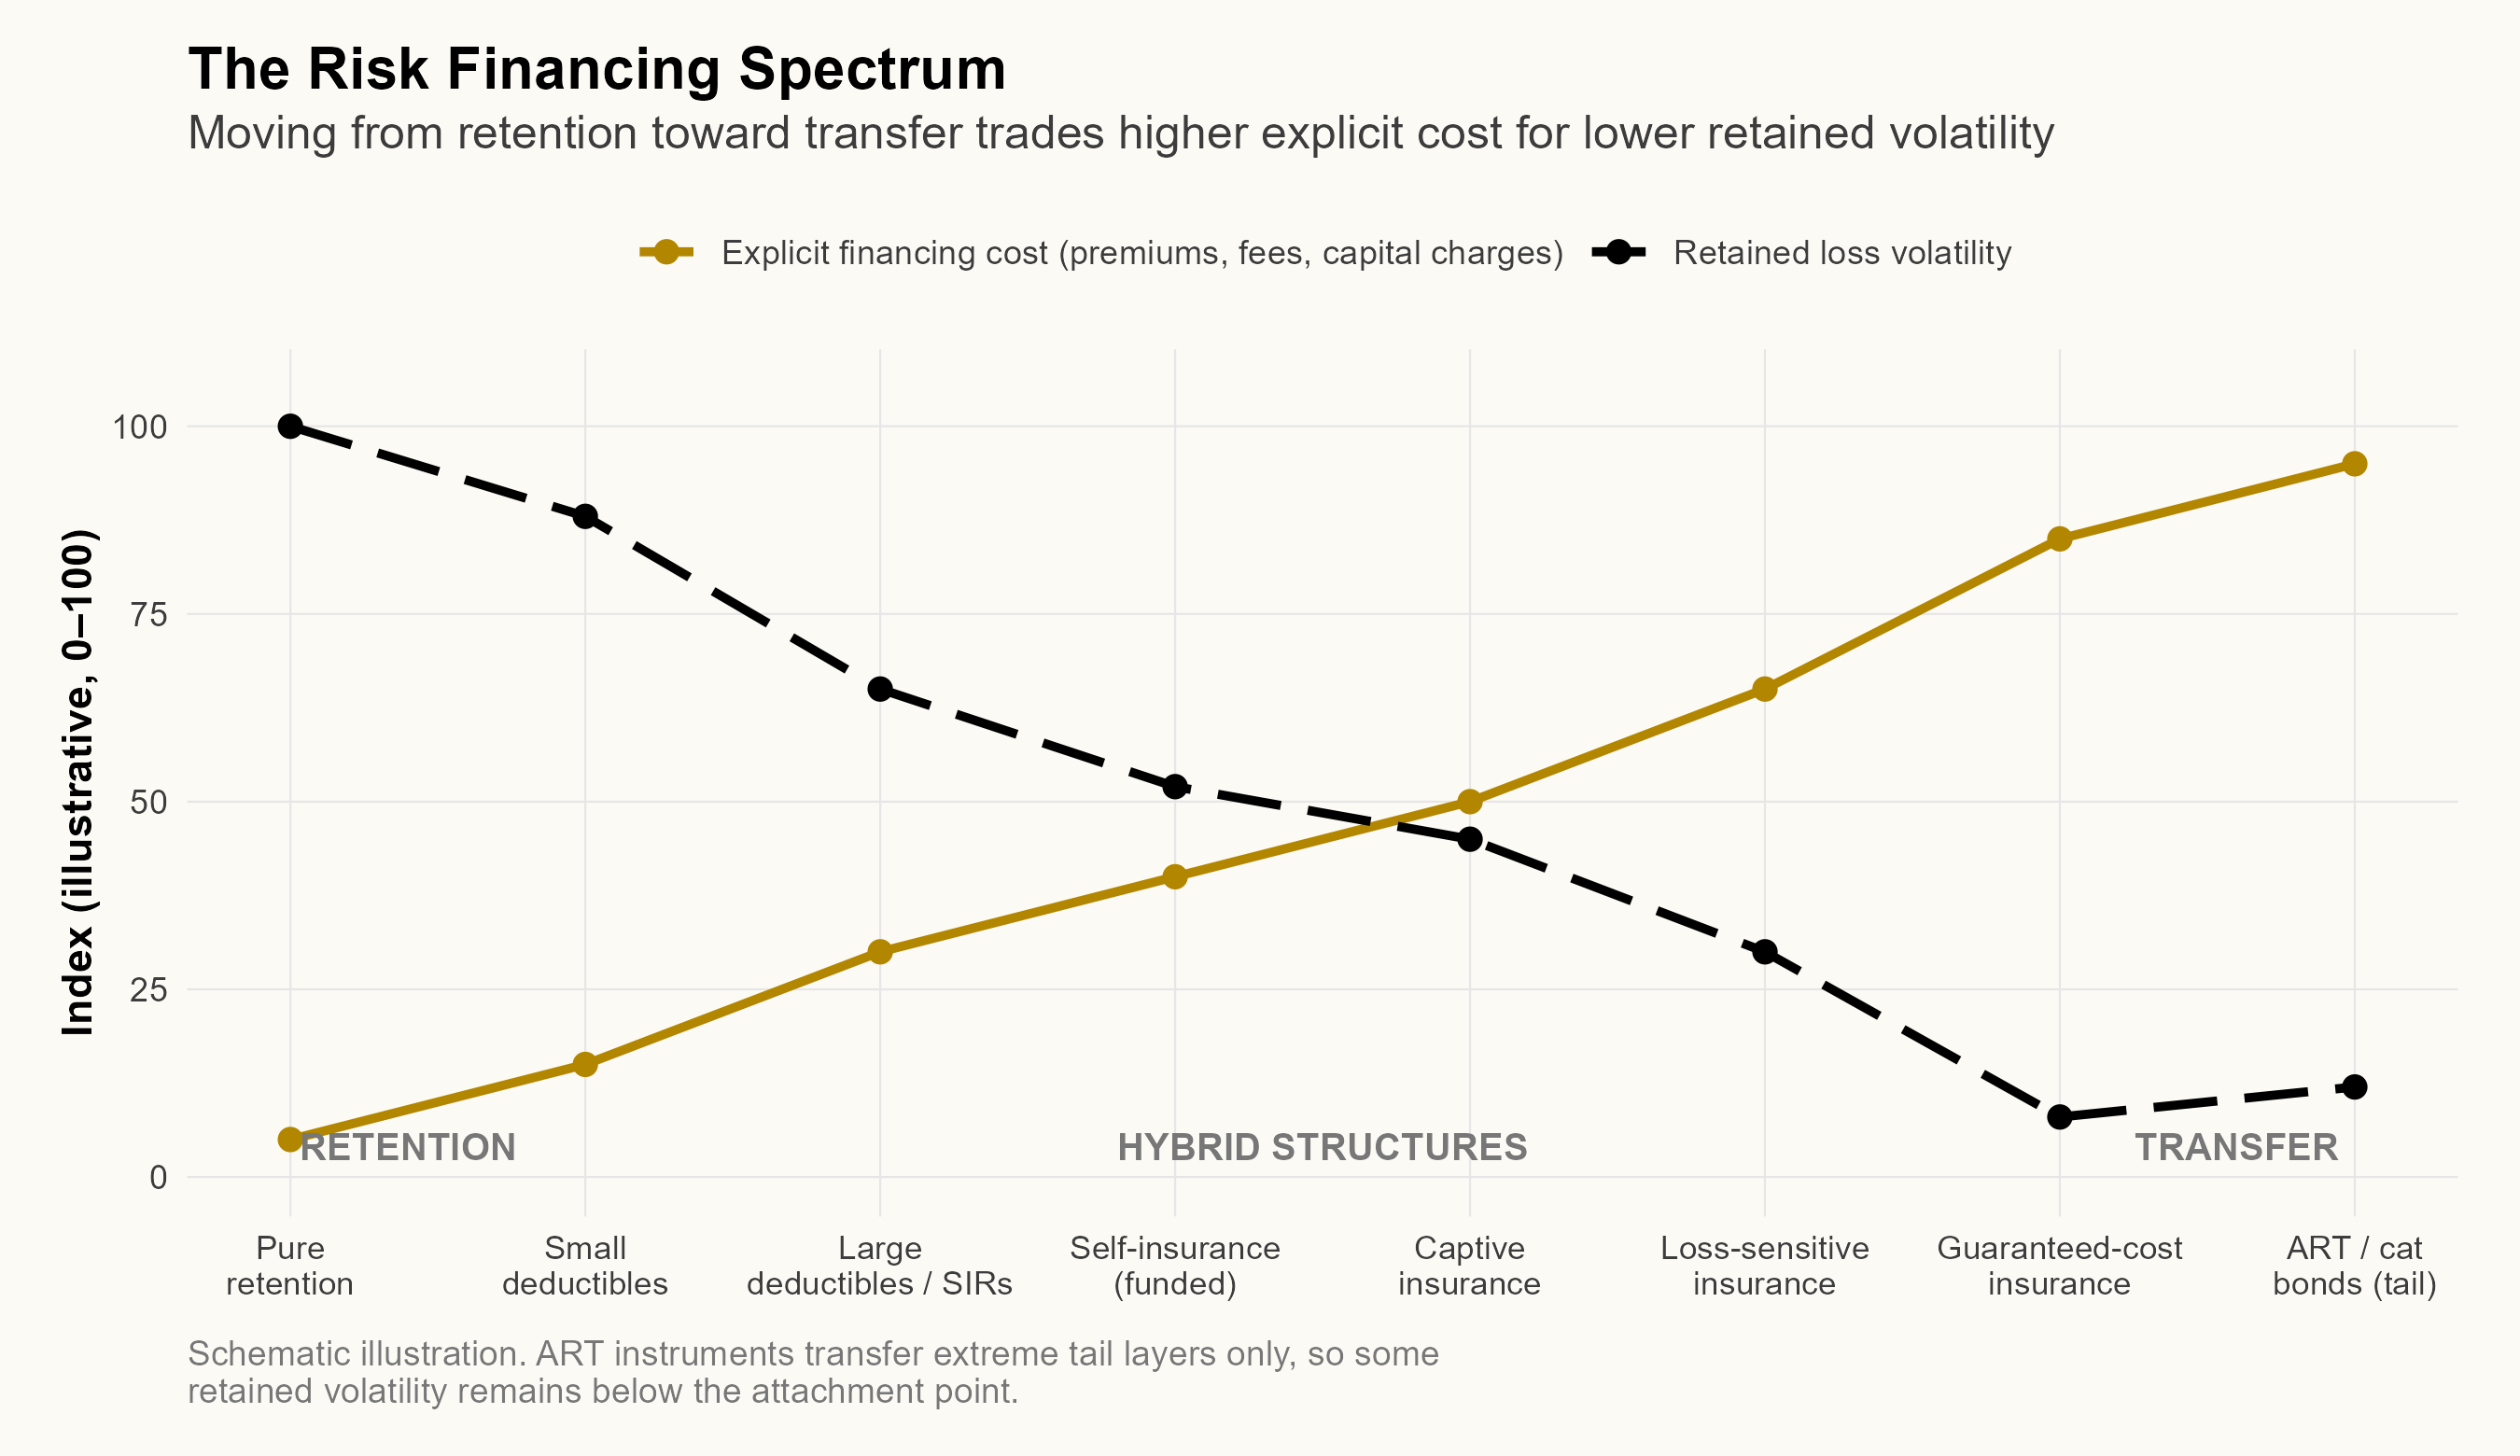
\includegraphics[width=\textwidth]{c8_financing_spectrum.png}
  \caption{The risk financing spectrum. Moving from retention toward transfer
  raises the explicit cost of financing and reduces retained loss volatility.
  ART instruments sit at the high-cost end but transfer only extreme tail
  layers, so some retained volatility remains below the attachment point.}
  \label{fig:spectrum}
  \figurenote{Schematic illustration; index values are illustrative rather
  than data. Generated by \texttt{rscripts/chapter8/c8\_financing\_spectrum.r}.}
\end{figure}

\textbf{Pure retention.}\index{risk retention} The organization absorbs all losses internally,
paying claims as they occur from operating cash flow or dedicated reserves.
Explicit cost is minimal (no premiums), volatility is maximal, and the
organization keeps complete control over claims.

\textbf{Small deductibles.} Most commercial policies include
deductibles\index{deductibles}---the amount the insured pays before insurance responds. Small
deductibles (\$10,000--\$50,000) reduce premiums modestly (5--15\%) while
eliminating nuisance claims that cost more to administer than they are worth.

\textbf{Large deductibles and SIRs.} Organizations with strong balance sheets
often choose retentions of \$250,000 to \$1 million or more per occurrence,
cutting premiums 30--50\% while retaining frequency exposure and transferring
severity. A \emph{self-insured retention (SIR)}\index{self-insured retention (SIR)} functions like a large
deductible with a legal distinction: under an SIR the insured pays claimants
directly before insurance attaches, whereas a deductible is typically
advanced by the insurer and reimbursed by the insured. SIRs are common in
liability lines, where direct payment reduces administrative friction.

\textbf{Funded self-insurance.} A formal program of retention backed by
actuarially determined reserves, professional claims administration, and
aggregate stop-loss protection (Section~\ref{sec:self-insurance}).

\textbf{Captive insurance.} The organization establishes its own licensed
insurance subsidiary to formally retain and manage risk while gaining tax,
regulatory, and reinsurance-access advantages (Section~\ref{sec:captives}).

\textbf{Loss-sensitive insurance.} Retrospectively rated programs and
dividend plans link the final premium to actual loss experience, blending
retention and transfer within a single policy
(Section~\ref{subsec:pricing-mechanics}).

\textbf{Guaranteed-cost insurance.} Fixed-premium coverage with no
loss-sensitive features provides maximum budget certainty: the insured knows
its exact insurance cost for the period regardless of losses, and pays the
highest expense load for the privilege.

\textbf{Alternative risk transfer.} Catastrophe bonds, sidecars, industry
loss warranties, and finite structures occupy the far end of the spectrum.
Note the wrinkle visible in Figure~\ref{fig:spectrum}: ART instruments
typically transfer only extreme tail layers, so some retained volatility
remains below the attachment point even as explicit cost peaks.

\subsection{The Cost--Volatility Tradeoff}
\label{subsec:cost-volatility}

Moving rightward along the spectrum costs more and retains less volatility.
The tradeoff\index{cost-volatility tradeoff} reflects an economic reality rather than an arbitrary pricing
convention: volatility reduction is a service, and the insurers and investors
who provide it require compensation for bearing risk and for their costs of
doing business.

Insurance premiums exceed expected losses by the expense load\index{expense load}:

\[
\text{Premium} = \text{Expected Loss} \times (1 + \text{Expense Load})
\]

where the load covers acquisition costs (agent and broker commissions,
marketing, underwriting---roughly 10--15\% of premium), administrative
expenses (claims adjustment, policy servicing, overhead---another 10--15\%),
and underwriting profit and contingencies (5--10\%) (Insurance Information
Institute, 2023). Expressed as a markup over expected losses rather than a
share of premium, typical commercial property-casualty loads run 25--40\%.

A concrete example. An organization with \$1 million in expected annual
property losses faces a premium of roughly \$1.4 million for ground-up
coverage---a 40\% markup, or \$400,000 of expense load. Suppose instead it
retains the first \$500,000 per occurrence through a large deductible.
Expected retained losses are \$600,000 (the frequent small claims account for
most expected loss), and the premium for excess coverage falls to
\$600,000---covering \$400,000 of expected transferred losses at a steeper
50\% markup, because excess layers carry proportionally higher loads. Total
cost falls from \$1.4 million to \$1.2 million: the organization saves
\$200,000 by no longer paying an expense load on losses it could finance
itself, and accepts the volatility of the retained layer in exchange.

The optimization logic generalizes. Retain predictable, high-frequency losses
where the law of large numbers makes outcomes nearly certain and the expense
load buys little; transfer unpredictable, low-frequency/high-severity
exposures where volatility reduction per premium dollar is greatest; and cap
the maximum retained loss so the program respects risk appetite.
Section~\ref{sec:tcor} formalizes this intuition as TCOR optimization.

\subsection{Factors Influencing Position on the Spectrum}

Organizations settle at different points on the spectrum for identifiable
reasons.

\textbf{Financial strength.} Large, profitable corporations with substantial
reserves and diversified operations gravitate toward retention; they can
absorb bad years without distress. Small businesses with limited capital must
transfer risks that could threaten solvency.

\textbf{Risk tolerance and culture.}\index{risk tolerance} From Chapter~5,
the risk appetite\index{risk appetite} framework constrains financing structure directly.
Conservative boards may mandate low retentions and comprehensive insurance
despite the higher cost, prioritizing earnings stability. Boards comfortable
with volatility may retain aggressively to minimize premium spend.

\textbf{Loss predictability.} Stable, high-frequency loss patterns support
confident retention---workers' compensation for a large employer with mature
safety programs is the standard example. Catastrophic exposures with low
frequency and devastating severity warrant transfer despite expensive
pricing; this is precisely where OLC landed on earthquake.

\textbf{Access to capital markets.} Publicly traded corporations with ready
access to equity and debt can finance retained losses through normal treasury
operations. Private companies, or firms near covenant limits, lack that
flexibility---for them insurance functions as contingent capital.

\textbf{Regulatory and contractual requirements.} States require proof of
financial responsibility for workers' compensation and auto liability;
lenders and counterparties routinely mandate insurance. These requirements
constrain retention regardless of what economic optimization would suggest.

\textbf{Tax considerations.} Premiums paid to qualified insurers are
immediately deductible; self-insured losses may face timing disadvantages.
Captives offer planning opportunities under anti-abuse scrutiny
(Section~\ref{subsec:captive-tax}).

\textbf{Management expertise and systems.} Sophisticated retention requires
claims systems, actuarial capability, and experienced staff. Organizations
without that infrastructure may rationally pay higher premiums for
administrative simplicity.

% =======================================================================
\section{Retention versus Transfer: The Core Decision}
\label{sec:retention-transfer}

\subsection{The Fundamental Cost Comparison}
\label{subsec:cost-comparison}

For any given exposure, the organization compares total expected costs\index{risk retention!versus transfer}:

\begin{align*}
\text{Total Cost of Retention} ={}& E[\text{Retained Losses}]
+ \text{Cost of Capital Held Against Losses} \\
&+ \text{Administrative Costs}
\end{align*}

\begin{align*}
\text{Total Cost of Transfer} ={}& \text{Insurance Premiums}
+ \text{Residual Retained Losses} \\
&+ \text{Brokerage and Fees}
\end{align*}

The decision minimizes total expected cost subject to risk appetite
constraints.

\textbf{Cost of retention.} Retaining risk requires capital held against
potential losses, and that capital has an opportunity cost at the firm's cost
of capital\index{cost of capital} \(k\). Required reserves typically equal expected losses plus a
safety margin tied to the loss distribution from
Chapter~4---for instance, reserves at the 95th
percentile:

\[
\text{Required Reserves} = E[\text{Losses}]
+ \big(\text{VaR}_{0.95} - E[\text{Losses}]\big) = \text{VaR}_{0.95}
\]

Suppose an organization expects \$2 million in annual losses with VaR(95\%)
of \$3.5 million, and its cost of capital is 10\%. The annual opportunity
cost of holding reserves at VaR is \(\$3.5\text{M} \times 0.10 =
\$350{,}000\). Adding expected losses of \$2 million and administrative costs
(claims handling, safety programs) of \$200,000:

\[
\text{Total Annual Cost of Retention}
= \$2{,}000{,}000 + \$350{,}000 + \$200{,}000 = \$2{,}550{,}000
\]

\textbf{Cost of transfer.} Full insurance for the same exposure, at a 35\%
expense load, costs \(\$2\text{M} \times 1.35 = \$2.7\) million in premium.
Adding broker fees of 5\% of premium (\$135,000) and roughly \$100,000 of
expected losses retained within small per-claim deductibles:

\[
\text{Total Annual Cost of Transfer}
= \$2{,}700{,}000 + \$135{,}000 + \$100{,}000 = \$2{,}935{,}000
\]

\textbf{Decision.} Retention costs \$2.55 million against \$2.935 million for
transfer---a saving of \$385,000 annually, about 13\%. But retention exposes
the organization to outcomes as bad as \$3.5 million (and worse, beyond the
95th percentile). If the board's risk appetite caps acceptable annual loss
volatility at \$3 million, retention is infeasible regardless of its expected
savings. The appetite constraint, not the cost comparison, is binding---a
pattern that recurs throughout this chapter.

\subsection{The Optimal Retention Level}
\label{subsec:optimal-retention}

Rather than choosing pure retention or pure transfer, most organizations
select a retention level\index{optimal retention level}---a deductible or SIR---that balances premium
savings against capital costs and appetite limits. Formally:

\[
\min_{R} \; \text{TCOR}(R) = E[L(R)] + k \cdot C(R) + P(R) + \text{Admin}(R)
\quad \text{s.t.} \quad \text{VaR}_{0.95}(R) \le \text{Appetite Limit}
\]

where \(R\) is the retention level, \(E[L(R)]\) the expected retained losses
at retention \(R\), \(C(R)\) the capital required to support that retention,
\(k\) the cost of capital, \(P(R)\) the premium for excess coverage above
\(R\), and \(\text{Admin}(R)\) administrative costs.

The comparative statics are intuitive. As \(R\) rises, expected retained
losses and required capital rise while premium falls; retained VaR rises
until it hits the appetite boundary. The optimum \(R^{*}\) is where marginal
premium savings stop covering the marginal cost of retained losses and
capital---or where the appetite constraint binds, whichever comes first.

\textbf{Worked example.} An organization faces property losses with expected
annual loss of \$1.5 million and a loss standard deviation of \$900,000. Its
cost of capital is 12\%, the insurer's expense load is 35\%, capital is held
at 150\% of expected retained losses, and the board's appetite limit is
VaR(95\%) \(\le\) \$4 million. Table~\ref{tab:retention-levels} evaluates
three candidate retentions.

\begin{ermtable}{Retention alternatives compared (\$000s)}[tab:retention-levels]
\begin{tabular}{@{}lrrrrrrr@{}}
\toprule
\textbf{Retention} & \textbf{Retained} & \textbf{Capital} &
\textbf{Cap.\ cost} & \textbf{Transferred} & \textbf{Premium} &
\textbf{Total} & \textbf{VaR(95\%)} \\
 & \textbf{loss} & \textbf{(150\%)} & \textbf{@12\%} &
\textbf{loss} & \textbf{@1.35\(\times\)} & & \\
\midrule
\$0 (full ins.) & 0 & 0 & 0 & 1{,}500 & 2{,}025 & 2{,}025 & \(\approx 0\) \\
\$500K & 400 & 600 & 72 & 1{,}100 & 1{,}485 & 1{,}957 & 2{,}800 \\
\$1M & 700 & 1{,}050 & 126 & 800 & 1{,}080 & 1{,}906 & 3{,}500 \\
\bottomrule
\end{tabular}
\tablenote{Premiums equal 1.35 times expected transferred losses; capital is
held at 150\% of expected retained losses with a 12\% opportunity cost.}
\end{ermtable}

Full insurance costs \$2,025K and eliminates volatility. The \$500K retention
saves \$68K annually (3.4\%) with retained VaR comfortably inside the limit.
The \$1M retention saves \$119K (5.9\%) and still respects the \$4M appetite.
The optimal retention is \$1M---the highest candidate whose VaR remains
inside appetite. Note what drives the result: every dollar of expected loss
moved from the transferred to the retained column saves its 35-cent expense
load but costs 18 cents of capital charge (150\% \(\times\) 12\%), so
retention wins on expected cost until the appetite constraint stops it.

\subsection{Decision Rules and Heuristics}

Quantitative optimization is the right framework, but practitioners lean on a
handful of rules that capture most of its content.

\textbf{Rule 1: Retain high-frequency, low-severity risks.} Frequent losses
with predictable severity are prime retention candidates---the law of large
numbers makes annual outcomes nearly certain, so the expense load buys
nothing. Fleet physical damage for a 500-vehicle company; employee health
claims for a large employer.

\textbf{Rule 2: Transfer low-frequency, high-severity risks.} Catastrophic
exposures that could threaten viability warrant transfer despite expensive
pricing. Product liability for a pharmaceutical manufacturer; earthquake for
a Tokyo Bay theme park; cyber breach liability for a retailer holding payment
card data.

\textbf{Rule 3: Cap retention by financial capacity.} A conservative rule of
thumb: maximum aggregate annual retention should not exceed 5--10\% of net
worth or 15--20\% of pre-tax earnings, so a bad year does not become a
distress event.

\textbf{Rule 4: Transfer non-core risks, retain core competencies.} Transfer
risks where insurers hold informational and claims-handling advantages
(directors and officers liability for an operating company). Retain risks
central to operations---product quality, employee safety---where the
organization controls outcomes better than any insurer could.

\textbf{Rule 5: Evaluate correlation in aggregate.} From
Chapter~6, retention decisions made line by line
ignore portfolio effects. Retaining several uncorrelated exposures is safer
than the line-by-line view suggests; retaining correlated ones is more
dangerous. Section~\ref{subsec:multiline} quantifies this.

% =======================================================================
\section{Traditional Risk Financing: Commercial Insurance}
\label{sec:commercial-insurance}

\subsection{The Insurance Value Proposition}

Insurance\index{commercial insurance} performs three economic functions that justify paying an expense
load rather than retaining.

\textbf{Risk pooling and diversification.}\index{risk pooling}\index{diversification} Insurers pool thousands or
millions of largely independent exposures, achieving diversification no
single insured can replicate. The law of large numbers\index{law of large numbers} makes the insurer's
aggregate outcome predictable even though each insured's outcome is not
(Rejda \& McNamara, 2017).

\textbf{Claims expertise.} Professional insurers bring specialized capability
in claims investigation, defense, and settlement that reduces total claim
cost: medical cost containment in workers' compensation, litigation
management in liability, negotiated repair networks in property. For complex
claims these savings can exceed the insurer's entire administrative fee
(Harrington \& Niehaus, 2004).

\textbf{Contingent capital.}\index{contingent capital} The insurer's promise to pay is pre-arranged
financing activated by loss events. For organizations with limited capital
market access or binding covenants, this contingent capital has value beyond
the loss payment itself (Froot et al., 1993)---the same economic function OLC
bought from bond investors, purchased instead from an insurer's balance
sheet.

\subsection{Major Commercial Insurance Lines}
\label{subsec:lines}

\textbf{Property insurance}\index{property insurance} covers direct physical damage to buildings,
equipment, and inventory from covered perils. Standard commercial forms use
``special form'' (all-risks) coverage---protection against everything except
specific exclusions, commonly flood, earthquake (both separately insurable),
war, and nuclear hazard (Insurance Services Office, 2012). Typical structures
include per-occurrence deductibles from \$5,000 to \$1 million or more,
limits set at insured values or blanket limits across locations, coinsurance
clauses requiring insurance to at least 80--90\% of value, and optional
business interruption coverage for lost income during restoration. Recall
from Chapter~3 that business interruption is an
operational/hazard exposure; the insurance that finances it rides on the
property form.

\textbf{Commercial general liability (CGL)}\index{commercial general liability (CGL)} provides third-party coverage for
bodily injury and property damage arising from premises, operations, and
products. CGL is written on an \emph{occurrence} basis\index{occurrence versus claims-made coverage}: coverage attaches
based on when the injury occurred, regardless of when the claim is filed,
creating long-tail exposure in which claims surface years after policy
expiration (Harrington \& Niehaus, 2004). Typical structures: per-occurrence
limits of \$1--5 million, general aggregate limits of \$2--10 million,
separate products/completed-operations aggregates, and defense costs paid in
addition to limits.

\textbf{Workers' compensation}\index{workers' compensation}, mandatory in most states, pays statutory
medical and wage-replacement benefits to injured employees while shielding
employers from tort liability under the exclusive remedy doctrine\index{exclusive remedy doctrine}. Because
benefits are prescribed by statute, loss patterns are comparatively
predictable---which is why workers' compensation is the most common line for
large-deductible programs and self-insurance (National Academy of Social
Insurance, 2021). Premiums adjust to the employer's own loss history through
the experience modification rate (EMR)\index{Experience Modification Rate (EMR)} introduced in
Chapter~7.

\textbf{Professional liability (errors and omissions)}\index{professional liability insurance} covers economic
damages from professional mistakes or failure to deliver promised
services---architects, engineers, accountants, consultants, technology
providers. Unlike occurrence-based CGL, professional liability is written on
a \emph{claims-made} basis\index{occurrence versus claims-made coverage}, covering only claims first made during the policy
period. The distinction matters when switching insurers or winding down
operations, when ``tail'' coverage must be purchased to cover claims not yet
reported.

\subsection{Insurance Pricing Mechanics}
\label{subsec:pricing-mechanics}

Actuaries build rates from the pure premium\index{pure premium}---expected loss per unit of
exposure:

\[
\text{Loaded Premium} = \text{Pure Premium}
\times (1 + \text{Expense Load})
\times (1 + \text{Profit and Contingency Margin})
\]

For property, the exposure base is \$100 of insured value; the pure premium
is historical loss cost per \$100, trended and adjusted for territory,
construction, protection class, and occupancy. A manufacturer insuring a \$10
million building might face a pure premium of \$0.25 per \$100 loaded to
\$0.34, for a total premium of \$34,000. For liability lines the exposure
base varies by classification---payroll for workers' compensation, sales for
products liability---and loads run higher (35--45\%) because of defense costs
and long claim durations.

Beyond fixed-price (``guaranteed cost'') policies, insurers offer
loss-sensitive structures that blend retention and transfer.

\textbf{Experience rating}\index{experience rating} adjusts premiums based on the insured's own
multi-year loss history. Workers' compensation experience rating through the
EMR is mandatory above a premium threshold; other lines offer credits and
debits at the underwriter's discretion.

\textbf{Retrospective rating}\index{retrospective rating} sets the final premium after the policy period
based on actual losses:

\[
\text{Retro Premium} = (\text{Basic Premium} + \text{Converted Losses})
\times \text{Tax Multiplier}
\]

subject to a minimum premium (often 60--70\% of standard) and a maximum
(often 125--140\%). The basic premium covers insurer overhead and profit;
converted losses are actual losses grossed up by a loss conversion factor
(typically 1.10--1.15) for claims-handling expense. The insured benefits
directly from good experience and is protected from catastrophic experience
by the maximum.

\textbf{Large-deductible and SIR programs}
(Section~\ref{subsec:optimal-retention}) reduce premiums to the cost of
excess coverage plus service fees.

\textbf{Dividend plans} return a portion of premium if losses run below
target thresholds---a profit-sharing arrangement common in workers'
compensation, where dividends of 20--40\% of premium are achievable for
excellent experience.

\subsection{Insurance Market Cycles: Hard and Soft Markets}
\label{subsec:market-cycles}

Insurance pricing is cyclical\index{insurance market cycle}, driven by industry capital and competitive
dynamics. In a \textbf{soft market}\index{soft market}, abundant capacity produces aggressive
pricing at or below actuarially indicated rates, broad coverage terms, and
readily available limits; insurer combined ratios drift above 100\% with
investment income covering the gap. In a \textbf{hard market}\index{hard market}, capital
impairment---from catastrophes or investment losses---produces rate increases
of 10--50\% or more at renewal, narrowed terms, withdrawn capacity, and
restored underwriting discipline.

Major hardenings followed September 11, 2001, Hurricane Katrina in 2005, and
the 2017--2021 period of heavy catastrophe losses capped by the pandemic. The
strategic implication for insureds: anticipate the cycle rather than chase
it. Organizations that slash retentions when coverage is cheap, then face
unaffordable renewals when the market turns, pay more over the cycle than
those that hold a stable program designed around their own risk-bearing
capacity (Insurance Information Institute, 2023). The market cycle is also a
standing argument for the alternative mechanisms in
Sections~\ref{sec:captives}--\ref{sec:securitization}, which insulate part of
the program from renewal repricing.

% =======================================================================
\section{Self-Insurance and Retention Programs}
\label{sec:self-insurance}

\subsection{Self-Insurance Fundamentals}

\textbf{Self-insurance}\index{self-insurance} is the deliberate, structured decision to retain risk
and pay losses from organizational resources. The word \emph{structured}
distinguishes it from ``going bare''---operating without coverage because
insurance seems expensive. A true self-insurance program incorporates
actuarial funding (reserves accumulated against projected losses), formal
claims administration, integrated safety and loss control, aggregate
protection capping extreme outcomes, and compliance with state financial
responsibility requirements.\footnote{Regulatory requirements for
self-insurance vary substantially by state and coverage type. Organizations
considering self-insurance should consult qualified advisors in every
jurisdiction where they operate.}

\subsection{When Self-Insurance Makes Economic Sense}

Five conditions favor self-insurance, and most successful programs satisfy
all of them.

\textbf{Scale and predictability.} Enough exposure units---employees,
vehicles, locations---that the law of large numbers operates internally.
Common benchmarks: 500+ employees for workers' compensation; 250+ vehicles
for auto liability.

\textbf{Financial capacity.} Balance sheet strength to absorb adverse years.
Rule of thumb: required reserves (expected losses plus 1.5--2.0 standard
deviations) should not exceed 15--20\% of net worth.

\textbf{Superior risk management.} Organizations that consistently outperform
industry loss averages subsidize weaker risks when they buy insurance priced
to the average. Self-insurance lets them keep the difference---the same logic
that justified Mercer Tool \& Stamping's loss control investment in
Chapter~7 carries over to financing.

\textbf{Expense load savings exceed administration costs.} Self-insurance
eliminates the insurer's 25--40\% load but adds internal or third-party
administration costs of roughly 5--15\% of losses. The net must be positive.

\textbf{Cash flow value.} Retaining cash until losses are paid, rather than
paying premiums in advance, benefits organizations whose investment
opportunities exceed the risk-free rate.

\subsection{Self-Insurance Program Structure}

\textbf{Funding mechanisms.} A \emph{pre-funded reserve account} accumulates
contributions equal to expected losses plus a margin, reaching steady state
at expected outstanding liabilities; for tax purposes, contributions are not
deductible---only paid losses are (26 U.S.C. \S~162). \emph{Pay-as-you-go}
funding pays claims from operating cash as they come due, maximizing cash
availability at the cost of volatile cash flows. To satisfy state security
requirements without tying up cash, organizations post \emph{letters of
credit} (bank fees of 1--3\% annually) or \emph{surety bonds} (2--5\% of face
amount).

\textbf{Claims administration.} Self-insureds must handle claims
professionally or pay for sloppiness in settlements, litigation, and
regulatory penalties. Three models: \emph{internal administration} (dedicated
staff---economic only for very large programs, roughly 5,000+ employees or
\$10M+ annual claims); \emph{third-party administrators (TPAs)}\index{third-party administrator (TPA)}, independent
firms that investigate, negotiate, and pay claims for fees of \$150--\$400
per claim or 8--12\% of incurred losses; and \emph{fronting arrangements}\index{fronting arrangement}, in
which a licensed insurer issues the policy and administers claims while the
insured retains the economic risk through deductible reimbursement
obligations.

\textbf{Aggregate stop-loss protection.}\index{aggregate stop-loss} Pure self-insurance leaves the
program exposed to a bad cluster of claims in a single year. Aggregate
stop-loss insurance caps annual retained losses at an attachment point,
typically 125--150\% of expected losses. An organization expecting \$3
million of workers' compensation losses might attach aggregate coverage at
130\%---\$3.9 million. If actual losses reach \$5 million, the stop-loss
insurer pays the \$1.1 million above the attachment. Premiums for the
aggregate layer typically run 5--15\% of the covered layer.

\subsection{Regulatory Requirements}

States regulate self-insurance to protect claimants---particularly injured
workers---from employers who retain risk without the capacity to pay.
Workers' compensation self-insurance typically requires state approval with
minimum net worth thresholds (\$1--25 million depending on state), audited
financials and actuarial certification of reserves, security deposits (cash,
letters of credit, or surety bonds scaled to payroll and loss history), proof
of specific and aggregate excess coverage, demonstrated claims administration
capability, and annual fees and assessments.

First-party property self-insurance is generally unregulated---the
organization bears the consequences of its own choices. Liability
self-insurance faces restrictions wherever third parties could be left
uncompensated: auto liability financial responsibility laws, environmental
bonding requirements for hazardous operations, and professional licensing
board requirements.

% =======================================================================
\section{Captive Insurance Companies}
\label{sec:captives}

\subsection{The Captive Concept}

A \textbf{captive insurance company}\index{captive insurance} is a licensed insurer owned and
controlled by its insureds, formed primarily to cover the risks of its parent
organization. A captive formalizes retention inside an insurance company
structure---with capital requirements, regulatory oversight, and professional
management---and in exchange gains the legal and economic standing of an
insurer. Roughly 7,000 captives operate worldwide, with U.S. corporations
accounting for about 40\% of formations (Captive Insurance Companies
Association, 2022).\footnote{Captive formation and operation require
compliance with domicile insurance regulation, federal and state tax law, and
parent-company accounting standards. Professional guidance from captive
managers, actuaries, tax counsel, and auditors is essential, and its cost
belongs in the captive feasibility analysis.}

Five defining characteristics: ownership by insureds rather than outside
shareholders; primary business of insuring parent risks; licensure and
regulation in a domicile jurisdiction; minimum capital and surplus
requirements; and professional underwriting, claims, actuarial, and
investment management.

The economic rationale parallels the value channels of
Section~\ref{subsec:value-channels}, applied through an insurance subsidiary.
The captive eliminates the commercial insurer's profit margin and overhead,
paying only incremental administration, regulatory, and reinsurance costs.
Premium paid to the captive accumulates as captive surplus and earns
investment income for the parent rather than for a commercial insurer---the
``float'' stays home. Premiums may be tax-deductible while the captive's
income enjoys favorable insurance company taxation
(Section~\ref{subsec:captive-tax}). The captive can write coverage that
commercial markets price punitively or refuse outright---terrorism, product
recall, brand protection, cyber---on terms the parent designs. And the
captive buys reinsurance directly at wholesale, skipping a layer of
intermediary loading.

\subsection{Types of Captive Structures}

\textbf{Single-parent (pure) captive.}\index{captive insurance!structures} Owned by one operating company to
insure its own risks; maximum control, but the parent funds all capital and
operating costs. Typical minimum capital: \$250,000--\$500,000 plus loss
reserves; annual operating costs \$75,000--\$200,000 for small captives and
\$250,000+ for sophisticated ones.

\textbf{Group captive.}\index{group captive} Owned by multiple unrelated organizations---usually
in the same industry---pooling homogeneous risks and sharing fixed costs.
Hospital systems pooling malpractice; contractors pooling workers'
compensation.

\textbf{Association captive.} Sponsored by a trade association for its
members; functionally a group captive or mutual with association governance.
Municipal workers' compensation pools and design-professional liability
captives are common examples.

\textbf{Protected cell company (PCC) / segregated portfolio company (SPC).}\index{protected cell company (PCC)} A
single licensed entity containing legally segregated ``cells,'' each with its
own assets and liabilities. Cells share infrastructure---cutting formation
cost---without sharing solvency. Cell rental runs \$25,000--\$75,000
annually, far below dedicated captive costs, making cells the entry point for
mid-sized firms.

\textbf{Rent-a-captive.} Participants rent underwriting capacity from an
existing captive---fastest market entry, least control.

\textbf{Agency captive.} Owned by an insurance agency to write its clients'
business. The structure creates obvious conflicts of interest (the broker
profits from placing business in its own captive) and draws regulatory
scrutiny.

\subsection{Captive Domicile Selection}

A captive must be licensed somewhere, and domiciles compete for formations on
regulation, tax, and cost\index{captive insurance!domicile selection}. \textbf{Vermont} is the oldest and largest U.S.
domicile (800+ captives), with a sophisticated regulator, deep
service-provider infrastructure, and a premium tax of 0.4\% capped at
\$200,000 for most captives. \textbf{Delaware} (roughly 400 captives) offers
no state premium tax and familiar corporate law. South Carolina, North
Carolina, Tennessee, and Utah market actively to home-state corporations.
Offshore, \textbf{Bermuda} (700+ captives) offers no corporate income tax,
respected regulation, and direct access to the world's largest reinsurance
market, at operating costs of \$150,000--\$300,000 annually and with U.S.
controlled-foreign-corporation tax complications; the \textbf{Cayman Islands}
is comparable with particularly flexible segregated portfolio legislation;
\textbf{Luxembourg, Ireland, and Malta} give EU passporting rights important
to multinationals with European operations.

Selection turns on tax treatment, regulatory quality, operating cost,
reinsurance access, proximity to the parent, legal infrastructure, and
political stability. In practice the choice is usually between the parent's
home-state domicile (administrative convenience, political goodwill) and a
major established domicile (depth of expertise).

\subsection{Tax Considerations}
\label{subsec:captive-tax}

Tax treatment can make or break captive economics\index{captive insurance!tax considerations}, and it attracts
correspondingly aggressive structuring and correspondingly aggressive
enforcement.

\textbf{Premium deductibility.} For premiums paid to a captive to be
deductible under 26 U.S.C. \S~162(a), the arrangement must be
\emph{insurance} in the sense of \emph{Helvering v.\ Le Gierse}\index{Helvering v. Le Gierse}, 312 U.S. 531
(1941) and its progeny, which requires both \textbf{risk transfer} (genuine
shifting of economic loss to the captive) and \textbf{risk distribution}\index{risk distribution}
(pooling across enough exposures for the law of large numbers to operate).
Single-parent captives insuring only the parent have historically struggled
with risk distribution. Accepted strategies include writing substantial
unrelated third-party business (often 30\%+ of premium), participating in
group structures or reinsurance pools, and insuring numerous operating
subsidiaries---though the IRS views brother-sister arrangements skeptically.

\textbf{The \S~831(b) election.}\index{831(b) election} ``Micro-captives'' with annual premiums at
or below the inflation-indexed limit (\$2.85 million for 2025) may elect
taxation on investment income only, paying no federal income tax on
underwriting income, provided diversification requirements are met (no more
than 20\% of premium from one insured). The election is legitimate for
genuinely operating small captives---and has been heavily abused by promoters
selling captives as estate-planning and tax shelters with token risk
transfer. The IRS designated certain micro-captive transactions as reportable
``listed transactions'' in Notice 2016-66; after that notice was set aside on
procedural grounds in litigation, the IRS finalized regulations in 2024
re-designating abusive micro-captive structures as listed transactions or
transactions of interest.\footnote{Genuine risk transfer, arm's-length
pricing, and adequate capitalization remain the touchstones; the procedural
litigation changed the disclosure mechanics, not the substantive
requirements.} The substance requirements are unchanged: real risk transfer,
arm's-length pricing, adequate capitalization, and a business purpose beyond
tax savings.

\textbf{Controlled foreign corporation rules.}\index{controlled foreign corporation (CFC) rules} Offshore captives owned by
U.S. parents are typically CFCs, and Subpart F (26 U.S.C. \S\S~951--965) can
pull insurance income into current U.S. taxation even if undistributed.
Exceptions exist for qualifying insurance income, but the analysis is
intricate and domicile-dependent---one reason the U.S. domiciles have grown
at the offshore centers' expense.

% =======================================================================
\section{Alternative Risk Transfer Instruments}
\label{sec:art}

\subsection{The ART Rationale}

\textbf{Alternative risk transfer (ART)}\index{alternative risk transfer (ART)} covers the non-traditional
mechanisms that blend insurance and capital market techniques, often
packaging multiple risks or multiple years into a single transaction. ART
emerged in the 1990s from a convergence of pressures: capacity crises that
made conventional coverage unavailable or unaffordable; corporate
dissatisfaction with one-year, one-line insurance pricing; the recognition
that global capital markets (measured in the hundreds of trillions of
dollars) dwarf the insurance industry's risk-bearing capacity (single-digit
trillions); and quantitative modeling advances that made bespoke structures
priceable. OLC's Midori bond is the cleanest illustration of the underlying
idea---when the risk is well-modeled and the traditional market is expensive,
go directly to investors.

\subsection{Finite Risk Insurance and Reinsurance}
\label{subsec:finite}

\textbf{Finite risk}\index{finite risk insurance} products cap the insurer's maximum loss at a modest
multiple of premium---typically 110--125\%---and explicitly price the time
value of money. Where traditional insurance transfers underwriting risk,
finite structures primarily transfer \emph{timing} risk, smoothing losses
over multi-year horizons.

Key features: premiums set well above expected losses (often 150--200\%),
with the excess accumulating in an \textbf{experience account}\index{experience account} that earns
interest at contractual rates; multi-year terms of 3--10 years; and
profit-sharing at expiry---favorable experience returns the account balance
to the cedent, adverse experience requires additional premium up to a cap,
and only losses beyond the cap land on the insurer.

\textbf{Example structure.} Calloway Industries\index{Calloway Industries} purchases five-year finite
reinsurance for product liability: annual premium \$2 million (\$10 million
total), expected losses \$6 million over the term, maximum insurer payout
\$12 million (120\% of premium), and a 4\% annual interest credit. Each year
the experience account grows by premium plus interest and is drawn down by
paid losses. At expiry, a positive balance is refunded; a deficit up to \$2
million is repaid by Calloway; anything beyond that cap is the reinsurer's
loss.

Finite risk serves loss smoothing (converting volatile annual outcomes into a
predictable multi-year cost---attractive to public companies managing
earnings guidance), structured funding of long-tail reserves, and regulatory
capital relief for insurers and banks.

The accounting deserves the caution it has earned\index{finite risk insurance!accounting issues}. To qualify for insurance
accounting, a finite contract must transfer genuine risk---both underwriting
and timing risk---under FASB ASC 944; structures that fail the test are
deposits, not insurance. Finite transactions were central to accounting
scandals at AIG and Gen Re in the early 2000s, where contracts with
negligible risk transfer were booked as reinsurance to dress up reserves.
Regulators have scrutinized the product line closely ever since.

\subsection{Multi-Trigger and Integrated Risk Programs}

\textbf{Multi-trigger policies}\index{multi-trigger policies} pay only when two or more specified events
occur together, cutting the probability of payout---and the
premium---relative to single-trigger coverage. Lakeshore Power \& Light\index{Lakeshore Power and Light}, a
utility, buys earthquake coverage that pays only if (1) an earthquake of
magnitude 7.0 or greater strikes its service territory \emph{and} (2) its
stock price falls 25\% or more within 30 days. The double trigger prices at
perhaps 40--60\% of conventional earthquake coverage. The logic is the
financial-distress channel from Section~\ref{subsec:value-channels}: the
company needs external capital only when physical damage coincides with
impaired financing capacity. If the earthquake comes and the stock holds,
treasury operations can fund the repairs.

\textbf{Integrated risk programs}\index{integrated risk programs} combine traditionally separate
lines---property, casualty, marine, political risk, business
interruption---into one policy with an aggregate retention and limit.
Meridian Industrial Group\index{Meridian Industrial Group} consolidates five lines into a single \$500 million
program with a \$50 million aggregate deductible across all perils. Because
the covered perils are imperfectly correlated (the
Chapter~6 logic, applied to insurance purchasing),
the integrated program prices 15--25\% below the sum of standalone policies.
Integrated programs suit multinationals with genuinely diversified exposures;
administrative complexity and jurisdictional insurance requirements limit
broader adoption.

\subsection{Risk Retention Groups}

The federal \textbf{Liability Risk Retention Act of 1986}\index{Liability Risk Retention Act} (15 U.S.C.
\S\S~3901--3906) authorizes \textbf{risk retention groups (RRGs)}\index{risk retention group (RRG)}---liability
insurers owned by their policyholder-members---to operate nationwide under a
single state license, preempting other states' licensing requirements (though
not their solvency oversight). The Act responded to the liability crisis of
the mid-1980s, when entire professions faced unavailable or unaffordable
coverage.

RRGs are restricted to liability lines (no property or workers'
compensation), require member ownership and industry homogeneity, and in some
structures impose joint and several liability among members---an arrangement
that concentrates the mind on underwriting discipline. Roughly 240 RRGs
operate today, concentrated in medical malpractice, product liability, and
commercial auto (National Association of Insurance Commissioners, 2023). They
function well for stable, homogeneous member bases; failures have generally
traced to underpricing or under-reserving in the early years, the standard
failure mode of mutual insurance.

% =======================================================================
\section{Risk Securitization: Catastrophe Bonds and Insurance-Linked
Securities}
\label{sec:securitization}

\subsection{The ILS Market}

\textbf{Insurance-linked securities (ILS)}\index{insurance-linked securities (ILS)} are financial instruments whose
payoffs depend on insurance loss events, transferring risk from insurers,
reinsurers, corporations, and governments to capital market investors. From
experimental transactions in the mid-1990s, the ILS market has grown into a
mature asset class exceeding \$100 billion, providing essential capacity for
catastrophic risk (Swiss Re, 2023).\footnote{The ILS market's modern growth
dates to the capacity shortage after Hurricane Andrew (1992) and accelerated
after Hurricane Katrina (2005). Structures, triggers, and covered perils
continue to evolve.}

The economics work for both sides. Sponsors gain access to risk-bearing
capacity that vastly exceeds the reinsurance industry's capital, particularly
for the low-frequency, high-severity perils---hurricane, earthquake,
pandemic---where reinsurance capacity is scarcest and most cyclical.
Investors gain an asset whose returns are driven by hurricanes and
earthquakes rather than by interest rates and corporate earnings: near-zero
correlation with equity and bond markets makes ILS a genuine diversifier even
at moderate expected returns (Cummins \& Weiss, 2009). When OLC issued the
Midori notes, it was renting exactly this: balance sheet capacity from
investors who held Japanese earthquake risk as one uncorrelated line in a
diversified portfolio.

\subsection{Catastrophe Bonds}
\label{subsec:catbonds}

\textbf{Catastrophe bonds}\index{catastrophe bond} are the largest ILS segment, with roughly \$45
billion outstanding. The structure deserves careful study because every
element solves a specific contracting problem.

The \textbf{sponsor}---an insurer, reinsurer, corporation, or government
seeking protection---enters a risk transfer agreement with a \textbf{special
purpose vehicle (SPV)}\index{special purpose vehicle (SPV)}\index{catastrophe bond!structure}, an independent entity (typically Bermuda or Cayman
domiciled) created for the transaction; Midori Ltd.\ played this role for
OLC. The SPV issues notes to investors and deposits the proceeds in a
\textbf{collateral trust}\index{collateral trust} invested in high-quality assets such as Treasury
money market funds. The sponsor pays the SPV a periodic premium. Investors
receive a floating coupon---the collateral yield (a money market rate such as
SOFR) plus the \textbf{risk spread} funded by the sponsor's premium, with
spreads typically 300--1,000 basis points depending on modeled risk. If no
trigger event occurs during the term, the collateral returns to investors at
maturity. If the trigger fires, collateral flows to the sponsor and investors
lose principal, in part or in whole.

Note the cost structure: because the collateral itself earns the money market
rate, the sponsor's economic cost is the risk spread, not the entire coupon.
This becomes important when comparing cat bond costs to reinsurance
rate-on-line (Section~\ref{subsec:reit-case}).

Two features distinguish the cat bond from reinsurance with the same limit.
First, the protection is \emph{fully collateralized}---the money exists in
trust on day one, eliminating the counterparty credit risk that haunts
reinsurance recoverables after a market-wide catastrophe. Second, the term is
multi-year (typically 3--5 years), locking in pricing across the reinsurance
cycle.

\textbf{Example transaction.} A Florida property insurer sponsors a \$300
million, 3-year cat bond paying SOFR + 650 basis points, triggered if modeled
industry losses from a Florida hurricane exceed \$50 billion. With SOFR at
4\%, investors earn 10.5\% running yield. Suppose catastrophe models from
firms such as Moody's RMS or Verisk put the annual trigger probability at
2\%. The investor's expected one-year return, assuming the full coupon is
received and principal is lost only in a trigger year:

\[
E[R] = 0.98 \times 10.5\% + 0.02 \times (-100\% + 10.5\%) \approx 8.3\%
\]

The 2\% expected loss of principal consumes about a fifth of the 10.5\%
coupon, leaving an expected return well above comparably rated corporate
credit---compensation for bearing tail risk that arrives suddenly and totally
rather than through gradual credit deterioration.

\subsection{Trigger Mechanisms}
\label{subsec:triggers}

Trigger design\index{catastrophe bond!triggers} is the central engineering problem in a cat bond, balancing
\textbf{basis risk}\index{basis risk} (the gap between what the sponsor loses and what the bond
pays) against \textbf{moral hazard}\index{moral hazard} (the sponsor's ability to influence
whether the bond pays).

\textbf{Indemnity triggers}\index{indemnity trigger} pay based on the sponsor's actual losses---zero
basis risk, maximum moral hazard, and slow settlement while losses develop.
Investors demand extra spread for the information asymmetry.

\textbf{Industry loss triggers}\index{industry loss trigger} pay when aggregate industry losses, as
estimated by an independent reporting agency such as PCS, exceed a threshold.
The sponsor cannot manipulate industry-wide losses, but its own experience
may diverge from the industry's---basis risk in both directions.

\textbf{Parametric triggers}\index{parametric trigger} pay based on measured physical parameters:
earthquake magnitude and location, hurricane central pressure, wind speed at
defined stations. This was the Midori design---payment determined entirely by
seismograph readings at specified monitoring points. Parametric triggers
eliminate moral hazard and settle fast (no loss adjustment, no negotiation;
OLC's collateral moved within weeks), at the price of the largest basis risk:
the instrument pays on physics, not on damage. OLC's risk team accepted that
tradeoff knowingly, and the 2011 event happened to land on the right side of
it---the recorded ground motion crossed the contractual thresholds \emph{and}
the liquefaction damage was severe. A slightly different earthquake could
have produced heavy damage without a triggering reading, leaving OLC with
losses and no recovery. Basis risk did not disappear because the bond paid;
it simply did not bind that day.

\textbf{Modeled loss triggers}\index{modeled loss trigger} run the event's physical parameters through a
pre-agreed catastrophe model to estimate losses, splitting the difference
between parametric simplicity and indemnity accuracy. Modeled and industry
triggers together account for the majority of recent issuance, with indemnity
triggers regaining share among insurer sponsors whose investors have grown
comfortable with their data.

\subsection{Other Insurance-Linked Securities}

\textbf{Collateralized reinsurance}\index{collateralized reinsurance}---economically similar to cat bonds but
documented as reinsurance contracts with the investor's capital posted in
trust---is now larger than the cat bond market itself (roughly \$50--60
billion), though private and less transparent. \textbf{Industry loss
warranties (ILWs)}\index{industry loss warranty (ILW)} are derivative contracts paying a fixed amount if
industry-wide losses exceed a threshold---\$10 million if PCS California
earthquake losses exceed \$50 billion, say---used mainly by reinsurers for
portfolio hedging; because payment is fixed rather than loss-based, there is
no adjustment process at all. \textbf{Mortality and longevity bonds}\index{mortality and longevity bonds}
securitize the two sides of life-contingent risk: mortality bonds pay
sponsors if deaths exceed a trigger (pandemic protection), longevity bonds
pay if populations live longer than expected (pension risk transfer); the
life ILS market remains small (\$10--15 billion) but growing.
\textbf{Sidecars}\index{sidecar} are temporary reinsurance vehicles capitalized by investors
to write quota-share business alongside a sponsor for 1--3 years---a fast way
to scale capacity in hard markets, with formations surging after Katrina, the
2017--2018 catastrophe years, and the pandemic.

\subsection{Advantages and Limitations of ILS}
\label{subsec:ils-advantages}

The advantages are real. \emph{Multi-year committed capacity} insulates
sponsors from renewal repricing. \emph{Non-correlating capital} means ILS
capacity survives insurance-market capital depletion---after a major
catastrophe, capital markets can replenish faster than reinsurer balance
sheets. \emph{Collateralization} eliminates counterparty credit risk.
\emph{Transparent pricing} through secondary trading (thin, but real) gives
both sides a market reference. And \emph{settlement speed}---for parametric
structures especially---delivers cash when it is worth the most; OLC was
financing reconstruction while a conventional claim would still have been in
the documentation stage.

The limitations are equally concrete. \emph{Basis risk} is the headline cost
of non-indemnity triggers, as Section~\ref{subsec:triggers} discussed.
\emph{Transaction costs}---structuring, legal, modeling, rating---run
\$500,000 to \$2 million per issuance, which is why cat bonds below \$100
million are uncommon. \emph{Lead time} of 3--6 months rules out ILS for
immediate capacity needs. \emph{Peril concentration}: securitization requires
credible models, so the market concentrates in well-modeled perils
(hurricane, earthquake, increasingly severe convective storm); cyber and
terrorism remain mostly beyond its reach. The instrument is a precision tool,
not a general substitute for insurance.

% =======================================================================
\section{Total Cost of Risk Optimization}
\label{sec:tcor}

\subsection{The TCOR Framework}

\textbf{Total cost of risk (TCOR)}\index{total cost of risk (TCOR)} aggregates every cost the organization
bears because risk exists, providing the common currency in which alternative
financing strategies are compared. Following the RIMS framework (RIMS,
2008):\footnote{Total cost of risk definitions vary among practitioners. The
RIMS framework includes retained losses, transfer costs, administrative
expenses, and certain indirect costs; organizations may add components such
as the cost of risk capital depending on their sophistication and
circumstances.}

\begin{align*}
\text{TCOR} ={}& \text{Retained Losses} + \text{Risk Transfer Costs}
+ \text{Administrative Costs} \\
&+ \text{Indirect Costs} + \text{Cost of Risk Capital}
\end{align*}

Retained losses include deductible and self-insured payments, claims-handling
costs on retained claims, and adverse development on prior years' retained
reserves. Risk transfer costs include premiums across all lines, collateral
costs (letters of credit, surety bonds), captive reinsurance, and ILS
spreads. Administrative costs cover the risk management department, TPAs,
brokers, actuaries, legal fees, and claims audits. Indirect costs---lost
productivity, management time, disruption---are the hardest to measure and
the most often omitted; Chapter~7's iceberg discussion
applies with equal force here. The cost of risk capital is the opportunity
cost of capital held against retained losses, plus regulatory and rating
agency capital effects for financial institutions.

\subsection{TCOR Benchmarking}

Industry surveys report median TCOR\index{total cost of risk (TCOR)!benchmarking} as a percentage of revenue: roughly
0.4--0.8\% for manufacturing, 1.5--3.0\% for healthcare (malpractice-driven),
2.0--3.5\% for construction, 0.2--0.5\% for financial services, and
1.5--2.5\% for transportation. An organization far above its industry median
is over-insuring, managing claims poorly, or experiencing loss frequency and
severity its controls should have prevented. An organization far below the
median is either genuinely superior or quietly under-insured---a distinction
that surfaces only in the tail, which is why benchmarking complements but
never replaces the appetite analysis of Chapter~5.

\subsection{The Optimization Model}

The retention optimization of Section~\ref{subsec:optimal-retention}
generalizes to the full program\index{total cost of risk (TCOR)!optimization}:

\[
\min_{R} \; \text{TCOR}(R) = E[L_{\text{ret}}(R)] + P(R) + \text{Admin}(R)
+ k \cdot C(R)
\quad \text{s.t.} \quad \text{VaR}_{0.95}(R) \le \text{Appetite}
\]

Each component responds to the retention level \(R\) in a characteristic way.
Expected retained losses rise with \(R\), steeply at first (the first layers
of retention absorb the high-frequency claims that carry most expected loss)
and then more slowly. Premium falls as coverage shrinks: with a 35\% load,
moving from full insurance on \$2 million of expected losses (premium \$2.7
million) to a retention that keeps \$400,000 of expected losses in-house cuts
the premium to \(\$1.6\text{M} \times 1.35 = \$2.16\) million---\$540,000 of
savings. Administrative costs are U-shaped: full insurance needs almost none,
heavy retention needs claims infrastructure, and moderate retention often
sits in the comfortable middle. The capital charge \(k \cdot C(R)\) rises
roughly in proportion to retained losses.

\subsection{A Worked Decision Table}
\label{subsec:decision-table}

Brennan Industrial Products\index{Brennan Industrial Products} evaluates five workers' compensation financing
strategies. Expected annual losses are \$2.0 million; the insurer's expense
load is 35\% on transferred expected losses; capital is held at 175\% of
expected retained losses with a 10\% cost of capital; and the aggregate
stop-loss premium under full self-insurance is \$400K.
Table~\ref{tab:brennan} shows the results (all figures in thousands). Each
premium equals 1.35 times the expected transferred losses (for the \$250K
deductible, \(1.35 \times \$1{,}400\text{K} = \$1{,}890\text{K}\)), so every
row can be reproduced from the assumptions.

\begin{ermtable}{Brennan Industrial Products: financing strategies compared
(\$000s)}[tab:brennan]
\small
\setlength{\tabcolsep}{4pt}
\begin{tabular}{@{}lrrrrrrr@{}}
\toprule
\textbf{Strategy} & \textbf{Retained} & \textbf{Premium} & \textbf{Admin} &
\textbf{Capital} & \textbf{Cap.\ cost} & \textbf{TCOR} & \textbf{VaR(95\%)} \\
 & \textbf{loss} & & & \textbf{held} & \textbf{@10\%} & & \\
\midrule
Guaranteed cost & 0 & 2{,}700 & 50 & 0 & 0 & \textbf{2{,}750} & \(\approx 0\) \\
\$250K deductible & 600 & 1{,}890 & 120 & 1{,}050 & 105 & \textbf{2{,}715} & 1{,}200 \\
\$500K deductible & 900 & 1{,}485 & 180 & 1{,}575 & 158 & \textbf{2{,}723} & 1{,}800 \\
\$1M SIR & 1{,}350 & 878 & 220 & 2{,}363 & 236 & \textbf{2{,}684} & 2{,}600 \\
Self-ins.\ + agg.\ stop-loss & 2{,}000 & 400 & 320 & 3{,}500 & 350 &
\textbf{3{,}070} & 3{,}200 \\
\bottomrule
\end{tabular}
\tablenote{Expected annual losses \$2.0M; premiums at a 1.35 load on expected
transferred losses; capital at 175\% of expected retained losses; cost of
capital 10\%.}
\end{ermtable}

The reading of this table repays attention. Unconstrained, the \$1M SIR
minimizes TCOR at \$2,684K---a \$66K saving over full insurance. But suppose
the board's appetite caps retained VaR(95\%) at \$2 million. The \$1M SIR
(VaR \$2.6M) and full self-insurance (VaR \$3.2M) are infeasible, and the
constrained optimum is the \$250K deductible at \$2,715K. The appetite
constraint costs \(\$2{,}715\text{K} - \$2{,}684\text{K} = \$31\text{K}\) per
year---a price worth making explicit, because it tells the board exactly what
its conservatism costs and invites a considered judgment about whether the
protection is worth it. Note also that full self-insurance is dominated here:
the premium saved no longer covers the capital charges and administration.
More retention is not always better, even before the appetite constraint
bites.

Sensitivity analysis matters as much as the base case. The \$250K and \$500K
deductibles differ by only \$8K---well inside estimation error---so the
choice between them turns on capital availability and administrative appetite
rather than on the point estimates. And if actual losses ran 20\% below
expectations, the rankings would shift toward higher retention. Model
multiple scenarios before committing.

\subsection{Multi-Line Portfolio Optimization}
\label{subsec:multiline}

Optimizing each line separately leaves money on the table, because
line-by-line analysis ignores the diversification\index{diversification} at the heart of
Chapter~6. If property and liability losses correlate
at 0.3 rather than 1.0, the volatility of the combined retained portfolio is
much less than the sum of the parts, and the organization can safely retain
more in aggregate than line-by-line optima suggest.

Suppose independent line analyses recommend retentions of \$500K (workers'
compensation), \$750K (property), and \$1M (liability)---\$2.25 million in
total. A portfolio analysis using the lines' correlation structure (workers'
compensation--property \(\rho = 0.4\), workers' compensation--liability
\(\rho = 0.2\), property--liability \(\rho = 0.5\)) shows that aggregate
retained VaR at these retentions sits well inside appetite, because the
lines' bad years do not coincide. Re-optimizing jointly supports roughly \$3
million of aggregate retention---about a third more---saving an additional
\$180K per year in expense loads. The portfolio view also corrects the
opposite error: lines that \emph{do} move together (the Maersk lesson from
Chapter~6---operational disruptions cascading across
what looked like separate exposures) should be retained more cautiously than
line-by-line analysis implies. Portfolio TCOR optimization requires actuarial
modeling of the joint loss distribution, but for organizations with several
material lines the savings are usually worth the modeling.

% =======================================================================
\section{Three Risk Financing Strategies}
\label{sec:cases}

The three cases in this section show the chapter's toolkit deployed under
different conditions: a financially strong manufacturer maximizing retention,
a hospital system escaping a failed commercial market through a group
structure, and a property owner blending reinsurance with capital markets.
The numbers in each case are internally consistent and worth working through
with a calculator.

\subsection{Case 1: GlobalTech Industries --- High Retention}
\label{subsec:globaltech-case}

\textbf{Profile.} GlobalTech Industries\index{GlobalTech Industries} is a \$12 billion revenue diversified
industrial manufacturer: 35,000 employees, 50 U.S. locations, 15
international facilities, \$4 billion of equity, investment-grade ratings,
and a mature safety program (TRIR 40\% below industry average). Its expected
annual losses: workers' compensation \$18M, property/business interruption
\$12M, product liability \$8M, auto liability \$3M---\$41M in total. The
board's appetite limits aggregate annual retained losses to \$75M at 95\%
confidence.

\textbf{Program.}

\emph{Workers' compensation:} \$1M per-occurrence deductible retaining \$14M
of expected losses (78\% retention); excess insurance from \$1M to \$25M for
\$5.5M premium; TPA fees \$0.6M. Annual cost \$20.1M against \$24M guaranteed
cost---a 16\% saving.

\emph{Property/BI:} \$5M per-occurrence retention with excess to \$250M;
expected retained \$8M; excess premium \$6.2M; captive administration \$0.5M.
Annual cost \$14.7M against \$17M---13\% saved.

\emph{Liability:} \$2M SIR with coverage to \$75M per occurrence / \$150M
aggregate; expected retained \$5M; premium \$4.8M; administration \$0.2M.
Annual cost \$10.0M against \$11.5M---13\% saved.

\emph{Auto liability:} \$250K per-occurrence deductible retaining \$2.5M of
expected losses; excess premium \$0.9M; TPA \$0.1M. Annual cost \$3.5M
against \$4.0M guaranteed cost---12.5\% saved.

\textbf{Program totals.} Expected retained losses \$29.5M; premiums \$17.4M;
administration \$1.4M; capital of \$50M held in the captive and corporate
reserves at an 8\% opportunity cost, \$4.0M.

\[
\text{TCOR} = \$29.5\text{M} + \$17.4\text{M} + \$1.4\text{M} + \$4.0\text{M}
= \$52.3\text{M}
\]

or 0.44\% of revenue---below the manufacturing median of roughly 0.6\%. The
guaranteed-cost alternative would run \$57.0M (\$24M + \$17M + \$11.5M +
\$4M of premiums plus \$0.5M of broker and administrative costs), so the
retention program saves \$4.7M annually (8.2\%). Modeled portfolio VaR(95\%)
of \$68M sits inside the \$75M appetite.

\textbf{Rationale.} Financial strength, diversification across lines and
geographies (low correlations shrink the aggregate VaR, per
Chapter~6), and superior loss control (the firm
outperforms the industry experience that commercial rates are priced to) all
point the same direction. The Vermont captive formalizes the retention,
captures investment income on reserves, and buys reinsurance at wholesale.
The savings are recycled into further loss control---the
Chapter~7 feedback loop operating at enterprise scale.

\subsection{Case 2: MidState Health System --- Group Captive for Malpractice}
\label{subsec:midstate-case}

\textbf{Profile.} MidState Health System\index{MidState Health System} operates eight hospitals with 2,500
affiliated physicians and \$1.8 billion of revenue. Its malpractice
experience: roughly 75 claims per year, of which about 60 settle below \$250K
(averaging \$15K---mostly incidents resolved without litigation) and about 15
are significant claims averaging \$850K in total severity. A five-year hard
market drove its commercial malpractice premium to \$22M while carriers cut
limits from \$5M to \$3M per occurrence---more money for less protection,
with two carriers exiting the state outright.

\textbf{Structure.} MidState joined five comparable regional systems to form
a Vermont-domiciled risk retention group\index{risk retention group (RRG)}. Each member contributed \$5M of
capital (\$30M total) and owns one-sixth of the RRG. The RRG writes each
member's coverage from \$250K to \$3M per occurrence (\$15M annual aggregate
per member) and buys group reinsurance from \$3M to \$10M per occurrence.
Members retain the first \$250K of every claim.

\textbf{MidState's annual economics.}
\begin{itemize}\tightlist
  \item Retained losses below \$250K: 60 claims \(\times\) \$15K =
        \textbf{\$0.9M}
  \item Expected ceded losses to the RRG layer: 15 claims \(\times\)
        (\$850K \(-\) \$250K) = \$9.0M; risk-allocated premium to the RRG:
        \textbf{\$10.5M} (an expected loss ratio near 86\%, leaving margin
        for the RRG's expenses)
  \item Share of the RRG's \$5M group reinsurance premium: \textbf{\$0.83M}
  \item TPA, legal, and internal risk management: \textbf{\$1.2M}
  \item Investment income on the \$5M capital commitment at 4\%:
        \textbf{\(-\$0.2\)M}
\end{itemize}

Total: \(\$0.9 + \$10.5 + \$0.83 + \$1.2 - \$0.2 = \$13.2\)M, against \$22M
of commercial premium for thinner limits---a saving of \$8.8M annually
(40\%), with per-occurrence protection to \$10M instead of \$3M.

\textbf{Why the pooling works.} Each member's annual losses have a standard
deviation of about \$7.8M. If the six members' losses were perfectly
correlated, the pool's standard deviation would be the simple sum, \$47M. At
the estimated inter-member correlation of 0.45 (members share
malpractice-environment and judicial-climate exposure but differ in geography
and specialty mix), the pooled standard deviation is

\[
\sigma_{\text{pool}} = 7.83 \times \sqrt{6 + 2 \times 15 \times 0.45}
\approx \$35\text{M},
\]

about 26\% below the perfectly correlated case---the
Chapter~6 aggregation formula doing the work that
makes group retention safe. The diversification lets the RRG hold a
substantial layer with confidence and buy reinsurance only for true excess
exposure.

\textbf{Five-year results.} The RRG ran a combined ratio near 92\%, returned
\$2M of dividends to members in years four and five, and grew surplus from
\$30M to \$55M---supporting higher retentions and cheaper reinsurance over
time. When the commercial market softened in year five, the RRG's pricing
simply held steady; members had exited the market cycle. Beyond the
financials, the RRG gave members governance control over underwriting and
claims philosophy, mandated patient-safety programs that improved underlying
loss experience, and created an anonymized benchmarking consortium.

\subsection{Case 3: Coastal Properties REIT --- Layered Reinsurance Plus Cat
Bond}
\label{subsec:reit-case}

\textbf{Profile.} Coastal Properties REIT\index{Coastal Properties REIT} holds \$3 billion of multifamily
real estate across Florida, South Carolina, and the Gulf Coast. Hurricane
modeling puts its 100-year probable maximum loss\index{probable maximum loss (PML)} at \$800M and its 250-year
PML at \$1.4B---concentrated, correlated exposure of exactly the kind
traditional markets price worst. After the 2017--2018 hurricane seasons,
reinsurance rates for coastal property rose 60--80\% and Gulf Coast capacity
contracted. A conventional quote---\$45M annually for \$500M of cover excess
of \$300M---amounted to 1.5\% of portfolio value per year, and the board
balked.

\textbf{The layered program.}

\emph{Layer 1 --- Retention, \$0--150M.} The REIT retains the working layer
through corporate resources and building-level policies. Expected annual
losses in the layer (tropical storms, tornadoes, hail): \$18M, plus \$0.4M of
administration.

\emph{Layer 2 --- Traditional reinsurance, \$150--450M.}\index{reinsurance!layered programs} Placed with a panel
of eight reinsurers for \$28M (a 9.3\% rate-on-line\index{rate-on-line}), covering moderate
hurricane scenarios.

\emph{Layer 3 --- Catastrophe bond, \$450--750M.} A 3-year, \$300M cat bond
through a Bermuda SPV with an industry-index trigger: 50\% of principal pays
out if PCS Florida hurricane losses exceed \$30B, 100\% above \$45B.
Investors receive SOFR + 725 basis points; since the collateral trust earns
SOFR, the REIT's annual cost is the spread:

\[
\$300\text{M} \times 7.25\% = \$21.8\text{M per year}
\]

for the three-year term.

\emph{Layer 4 --- Traditional reinsurance, \$750M--1B.} Extreme excess for
\$6M (2.4\% rate-on-line---cheap because attachment is remote).

\textbf{Total annual cost:} \$18M retained + \$34M reinsurance (Layers 2 and
4) + \$21.8M cat bond spread + \$2M administration and structuring
amortization = \textbf{\$75.8M}.

\textbf{The all-traditional comparison.} Covering the same \$150M--\$1B tower
entirely with reinsurance at a blended 8.5\% rate-on-line would cost
\(\$850\text{M} \times 0.085 = \$72.3\text{M}\) in premium, plus the same
\$18M of retained losses: \$90.3M in total. The layered program saves
\textbf{\$14.5M annually (16\%)}---and buys three years of locked pricing on
the cat bond layer while reinsurance renewals stayed turbulent.

\textbf{The basis risk decision.}\index{basis risk} The industry-index trigger means the bond
pays on PCS's Florida estimate, not on the REIT's own losses. The risk team
tested the index against its portfolio across 50 historical and modeled
hurricane scenarios and found 85\% correlation---high, because the
portfolio's geographic distribution resembles the state's insured property
distribution. They accepted the residual mismatch consciously, documented it
for the board, and sized Layer 2 (indemnity-based reinsurance) to carry the
scenarios where the index and the portfolio diverge most. This is the right
way to handle basis risk: measure it, price it, and place it where it is
least dangerous---not pretend it is absent. OLC made the same judgment with
its parametric trigger, and Section~\ref{subsec:triggers}'s caution applies
to both: the 2011 outcome validated OLC's design, but a near-miss earthquake
would have tested it.

\textbf{Outcome.} No qualifying hurricane struck during the bond's term;
investors recovered principal and the REIT renewed the bond at similar
pricing---cat bond spreads stayed stable while reinsurance quotes whipsawed.
Cumulative savings over five years exceeded \$70M against the all-traditional
alternative, and the rating agencies cited the program's structure favorably
in maintaining the REIT's credit rating.

% =======================================================================
% End-of-chapter material
% =======================================================================

\begin{keytakeaways}
\item
  \textbf{Risk financing completes the ERM cycle}: Loss control
  (Chapter~7) changes the loss distribution; risk
  financing decides who pays for what remains and when. The two are
  complements---financing structures like deductibles create the incentives
  that make loss control pay.
\item
  \textbf{The spectrum is a cost--volatility tradeoff}: From pure retention
  to guaranteed-cost insurance and ART, every step toward transfer raises
  explicit cost and lowers retained volatility. Optimal positioning retains
  predictable high-frequency losses (where expense loads buy nothing) and
  transfers low-frequency severity (where volatility reduction per dollar is
  greatest).
\item
  \textbf{Risk appetite, not expected cost, is usually the binding
  constraint}: Retention strategies routinely minimize expected TCOR but fail
  VaR limits. Computing the cost of the appetite constraint---the gap between
  the constrained and unconstrained optima---makes the price of conservatism
  explicit for the board.
\item
  \textbf{Self-insurance and captives are structured retention, not the
  absence of insurance}: They demand scale, capital, claims infrastructure,
  and aggregate protection; the captive adds a licensed structure that
  captures expense loads, investment float, reinsurance access, and (within
  anti-abuse limits) tax efficiency.
\item
  \textbf{ART instruments solve specific contracting problems}: Finite risk
  transfers timing risk; multi-trigger policies pay only when loss coincides
  with financing need; RRGs rebuild capacity that commercial markets
  abandoned. Each earns its complexity only when the targeted friction is
  material.
\item
  \textbf{Catastrophe bonds rent balance sheet from capital markets}: Fully
  collateralized, multi-year, and priced off the risk spread, they suit
  well-modeled tail perils. Trigger design trades basis risk against moral
  hazard---OLC's parametric bond paid within weeks precisely because it paid
  on physics rather than on adjusted losses, a design that would have carried
  real basis risk in a different earthquake.
\item
  \textbf{TCOR is the common currency, and the portfolio view pays}:
  Comparing strategies requires totaling retained losses, transfer costs,
  administration, and capital charges. Optimizing lines jointly rather than
  separately exploits the diversification mathematics of
  Chapter~6 and typically supports materially higher
  aggregate retention.
\end{keytakeaways}

% -----------------------------------------------------------------------
\begin{keyterms}
  \item[\keyterm{Aggregate stop-loss}] Insurance capping total retained
    losses across all events in a policy period, protecting self-insurers
    from adverse accumulations.
  \item[\keyterm{Alternative risk transfer (ART)}] Non-traditional risk
    financing mechanisms including finite reinsurance, catastrophe bonds,
    multi-trigger policies, and integrated risk programs.
  \item[\keyterm{Basis risk}] The difference between the sponsor's actual
    losses and an instrument's payout, arising whenever the trigger is
    anything other than the sponsor's own indemnified loss.
  \item[\keyterm{Captive insurance company}] A licensed insurer owned by its
    insureds to cover primarily the parent's risks, combining formal
    retention with insurance company structure.
  \item[\keyterm{Catastrophe bond (cat bond)}] An insurance-linked security
    transferring catastrophe risk to investors who lose principal if
    predefined triggers occur; proceeds are held in a collateral trust, and
    the sponsor's cost is the risk spread.
  \item[\keyterm{Collateralized reinsurance}] Reinsurance backed by investor
    capital posted in trust---economically similar to cat bonds but
    documented as private reinsurance contracts.
  \item[\keyterm{Deductible}] The amount of each loss the insured bears
    before insurance responds; the insurer typically advances payment and is
    reimbursed.
  \item[\keyterm{Expense load}] Insurer costs added to expected
    losses---acquisition, administration, profit, and
    contingencies---typically a 25--40\% markup in commercial
    property-casualty lines.
  \item[\keyterm{Experience account}] In finite risk contracts, the notional
    fund accumulating premiums plus interest and drawn down by losses, with
    the terminal balance shared between cedent and insurer.
  \item[\keyterm{Finite risk (re)insurance}] Multi-year structures capping
    the insurer's exposure at a modest multiple of premium and explicitly
    crediting investment income; transfers timing risk more than underwriting
    risk.
  \item[\keyterm{Fronting arrangement}] A licensed insurer issues the policy
    and administers claims while the insured retains the economic risk
    through deductible or reimbursement obligations.
  \item[\keyterm{Group captive}] A captive owned by multiple unrelated
    organizations pooling homogeneous risks.
  \item[\keyterm{Hard market}] The phase of the insurance cycle with depleted
    capacity, rising rates, and restrictive terms.
  \item[\keyterm{Industry loss warranty (ILW)}] A derivative paying a fixed
    amount if industry-wide losses from a specified peril exceed a threshold.
  \item[\keyterm{Insurance-linked securities (ILS)}] Instruments whose
    payoffs depend on insurance loss events---cat bonds, collateralized
    reinsurance, mortality and longevity bonds, sidecars.
  \item[\keyterm{Parametric trigger}] A payout condition defined by measured
    physical parameters (magnitude, wind speed, ground motion) rather than
    losses; fast settlement, maximal basis risk.
  \item[\keyterm{Protected cell company (PCC)}] A licensed entity containing
    legally segregated cells, letting multiple participants share captive
    infrastructure without sharing solvency.
  \item[\keyterm{Retention}] The portion of risk financed internally rather
    than transferred---via deductibles, SIRs, or aggregate retentions.
  \item[\keyterm{Retrospective rating}] Premium determined after the policy
    period from actual losses, bounded by minimum and maximum premiums.
  \item[\keyterm{Risk retention group (RRG)}] A policyholder-owned liability
    insurer authorized by federal law to operate nationwide under a single
    state license.
  \item[\keyterm{Self-insured retention (SIR)}] A retention the insured pays
    directly to claimants before coverage attaches; legally distinct from a
    deductible.
  \item[\keyterm{Self-insurance}] The structured decision to retain risk with
    actuarial funding, professional claims administration, and aggregate
    protection.
  \item[\keyterm{Sidecar}] A temporary investor-capitalized reinsurance
    vehicle writing quota-share business alongside a sponsor, typically for
    1--3 years.
  \item[\keyterm{Soft market}] The phase of the insurance cycle with abundant
    capacity, falling rates, and broad terms.
  \item[\keyterm{Third-party administrator (TPA)}] An independent firm
    providing claims services to self-insured organizations for fees.
  \item[\keyterm{Total cost of risk (TCOR)}] The sum of retained losses, risk
    transfer costs, administrative costs, indirect costs, and the cost of
    risk capital; the common metric for comparing financing strategies.
\end{keyterms}

% -----------------------------------------------------------------------
\begin{shortanswerquestions}
\item \textbf{TCOR comparison.} A manufacturer faces expected annual losses
  of \$1.8M. Full insurance costs \$2.5M in premium plus \$30K of broker
  fees. A \$500K-deductible program retains \$700K of expected losses, with
  an excess premium of \$1.45M, administrative costs of \$120K, and required
  capital of \$1.2M at a 10\% opportunity cost.
  \begin{enumerate}[label=\alph*)]\tightlist
    \item Calculate TCOR for full insurance.
    \item Calculate TCOR for the deductible program.
    \item What are the annual savings?
    \item What additional consideration might make the deductible infeasible
          despite the savings?
  \end{enumerate}
\item \textbf{Optimal retention with an appetite constraint.} Expected annual
  losses are \$2.2M; the insurer's load is 35\% on transferred expected
  losses; the cost of capital is 8\%.

  \begin{center}
  \begin{tabular}{@{}lrrrrr@{}}
  \toprule
  \textbf{Retention} & \textbf{Retained loss} & \textbf{Premium} &
  \textbf{Admin} & \textbf{Capital} & \textbf{VaR(95\%)} \\
  \midrule
  \$0 & \$0 & \$2,970K & \$40K & \$0 & \(\approx 0\) \\
  \$750K & \$900K & \$1,755K & \$150K & \$1,500K & \$2,400K \\
  \$1.5M & \$1,500K & \$945K & \$220K & \$2,500K & \$3,600K \\
  \bottomrule
  \end{tabular}
  \end{center}

  \begin{enumerate}[label=\alph*)]\tightlist
    \item Calculate TCOR for each retention level.
    \item Which retention is optimal if risk appetite limits retained
          VaR(95\%) to \$3M?
    \item Which is optimal if the limit is \$4M?
    \item What is the annual cost of the tighter appetite constraint?
  \end{enumerate}
\item \textbf{Cat bond expected return.} An investor buys a 3-year hurricane
  cat bond: principal \$100,000; coupon SOFR + 650 bp (take SOFR = 5\%, so
  the coupon is 11.5\%); annual trigger probability 3\%, independent across
  years; full principal loss if triggered. Assume the year's coupon is paid
  even in a trigger year.
  \begin{enumerate}[label=\alph*)]\tightlist
    \item Expected return in Year 1.
    \item Cumulative three-year return if the bond never triggers
          (compounded).
    \item Probability the bond survives all three years.
    \item At what annual trigger probability does the expected one-year
          return equal the 5\% risk-free rate?
  \end{enumerate}
\item \textbf{Self-insurance feasibility.} A 400-employee manufacturer
  (\$150M revenue) pays an \$800K workers' compensation premium (EMR 1.15).
  If self-insured: expected losses \$550K (SD \$200K), TPA costs \$90K,
  aggregate stop-loss premium \$40K (attaching at 130\% of expected losses),
  required reserves of expected losses plus 1.5 standard deviations, and a
  12\% opportunity cost of capital.
  \begin{enumerate}[label=\alph*)]\tightlist
    \item Calculate the total annual cost of self-insurance.
    \item Compare it to the current premium.
    \item Is this organization large enough to self-insure comfortably? What
          does the size of the margin suggest?
  \end{enumerate}
\item \textbf{Captive NPV.} A multinational with \$800M of global property
  values pays \$12M for property insurance with a 45\% expense ratio. A
  captive alternative would cost: \$250K formation (one-time), \$180K annual
  operations, \$600K annual reinsurance, \$500K of committed capital, and
  \$6.5M of expected retained losses annually.
  \begin{enumerate}[label=\alph*)]\tightlist
    \item Compute the captive's annual cost and the annual saving versus
          commercial insurance.
    \item Compute the five-year NPV of the captive at an 8\% discount rate
          (treat formation and capital as time-zero outlays; ignore capital
          recovery).
    \item Name three non-financial benefits the captive might add.
  \end{enumerate}
\end{shortanswerquestions}

% -----------------------------------------------------------------------
\begin{discussionquestions}
\item \textbf{Conceptual:} Explain the cost--volatility tradeoff along the
  risk financing spectrum. Why does volatility reduction command a price, and
  what economic principle underlies the expense load?
\item \textbf{Conceptual:} Describe the conditions under which retention
  beats transfer. Why does each condition matter, and which is most often the
  binding one in practice?
\item \textbf{Conceptual:} Distinguish deductibles from self-insured
  retentions legally and operationally. When would an organization prefer
  each?
\item \textbf{Conceptual:} What three economic functions justify insurance
  expense loads? Give an example of each.
\item \textbf{Conceptual:} Lay out the captive value proposition and its
  limits. Why do small organizations rarely benefit despite the advertised
  advantages?
\item \textbf{Conceptual:} Walk through the mechanics of a catastrophe
  bond---sponsor, SPV, collateral trust, trigger, spread. Why is the
  sponsor's economic cost the spread rather than the full coupon? Use the
  OLC/Midori transaction to illustrate.
\item \textbf{Conceptual:} Compare the four cat bond trigger types on basis
  risk, moral hazard, and settlement speed. Why did a parametric trigger suit
  OLC, and what risk did OLC accept in choosing it?
\item \textbf{Application:} Your organization buys \$5M of general liability
  coverage for \$350K (7\% rate-on-line). The market has been soft for three
  years; your broker expects hardening within two to three years, with rate
  increases of 30--50\%. Evaluate the tradeoffs among (a) staying the course,
  (b) negotiating a three-year policy at current rates, (c) raising retention
  to \$1M now, and (d) forming a captive. What would you recommend, and what
  does the timing depend on?
\item \textbf{Application:} Your risk portfolio includes workers'
  compensation (\$2.5M expected, \(\sigma\) = \$800K), property (\$1.8M
  expected, \(\sigma\) = \$1.2M), and liability (\$1.5M expected, \(\sigma\)
  = \$600K), with correlations WC--property 0.3, WC--liability 0.2,
  property--liability 0.4. Line-by-line optimization recommends retentions of
  \$1M (WC), \$500K (property), and \$750K (liability). Explain
  conceptually---no calculation required---why the portfolio view supports
  retaining more in aggregate, and what feature of the correlation matrix
  would reverse that conclusion.
\item \textbf{Application:} A coastal insurer needs \$200M of hurricane
  protection above a \$100M retention. Traditional reinsurance costs \$22M
  per year (11\% rate-on-line), pays on actual company losses, and renews
  annually. A 3-year cat bond pays a spread costing the sponsor \$26M per
  year, triggers on PCS Florida industry losses above \$35B, and carries an
  estimated 20\% basis risk. Which would you choose, and under what
  circumstances would the more expensive cat bond be preferable? Consider the
  market cycle, counterparty credit, collateralization, and what happens
  after a major industry loss.
\end{discussionquestions}

% -----------------------------------------------------------------------
\begin{minicase}{Cedar River Logistics --- Designing the Risk Financing
Program}

Cedar River Logistics\index{Cedar River Logistics} is a regional trucking and warehousing company: \$600
million in revenue, 2,800 employees, 1,400 power units, and 22 distribution
centers across the upper Midwest. The company currently buys guaranteed-cost
insurance for everything. The CFO suspects the program is expensive and has
asked you---the newly hired risk manager---to redesign it.

\textbf{Current program and loss data:}

\begin{center}
\begin{tabular}{@{}lrrr@{}}
\toprule
\textbf{Line} & \textbf{Expected loss} & \textbf{Loss SD} &
\textbf{Current premium} \\
\midrule
Auto liability & \$4.0M & \$1.5M & \$5.6M \\
Workers' compensation & \$2.5M & \$0.8M & \$3.5M \\
Cargo & \$1.2M & \$0.5M & \$1.7M \\
Cyber & \$0.8M & \$1.0M & \$1.3M \\
\midrule
\textbf{Total} & \textbf{\$8.5M} & & \textbf{\$12.1M} \\
\bottomrule
\end{tabular}
\end{center}

Correlations: auto--WC 0.4; auto--cargo 0.3; WC--cargo 0.2; cyber with all
other lines 0.1. The board's risk appetite limits aggregate retained losses
to \$9.0M at 95\% confidence. Cedar River's cost of capital is 9\%; assume
capital must be held at expected retained losses plus 1.5 portfolio standard
deviations of the retained book; assume insurers price excess coverage at a
35\% load on transferred expected losses; estimate TPA and administrative
costs for any retention program at 8\% of expected retained losses. For VaR
calculations, a normal approximation to the aggregate retained distribution
is acceptable.

\textbf{Your assignment (50 points):}

\begin{enumerate}
\item \textbf{Current-state TCOR (10 points).} Compute the TCOR of the
  guaranteed-cost program and express it as a percentage of revenue. Compare
  to the transportation industry benchmark of 1.5--2.5\%.
\item \textbf{Two alternative designs (25 points).} Design and price two
  alternatives:
  \begin{itemize}\tightlist
    \item \emph{Strategy A --- Retention program:} Select per-line retentions
      (state your assumed split of expected losses between retained and
      transferred layers, and keep the assumptions defensible). Compute
      expected retained losses, excess premiums, administrative costs, the
      capital charge, TCOR, and aggregate retained VaR(95\%) using the
      correlation matrix.
    \item \emph{Strategy B --- Retention plus one alternative mechanism:} Add
      a captive, group captive, or parametric/ART element to Strategy A for
      at least one line, and justify why that line suits the mechanism.
      Recompute TCOR and VaR.
  \end{itemize}
\item \textbf{Recommendation memo (15 points).} In no more than three pages,
  recommend a strategy to the CFO. State the TCOR savings, demonstrate
  appetite compliance, identify the two largest risks in your recommendation
  (e.g., adverse loss development, market cycle timing, basis risk), and
  propose one metric the board should monitor quarterly.
\end{enumerate}

\textbf{Deliverables:} the memo plus a spreadsheet showing all calculations
with formulas visible.
\end{minicase}

% -----------------------------------------------------------------------
\section*{References}
\addcontentsline{toc}{section}{References}
\begingroup
\sloppy
\begin{hangparas}{2em}{1}

Bermuda Monetary Authority. (2022). \emph{Insurance statistics report}.
Government of Bermuda. \url{https://www.bma.bm/}

Captive Insurance Companies Association. (2022). \emph{CICA international
captive domicile statistics}. \url{https://www.cicaworld.com/}

Cummins, J.~D., \& Weiss, M.~A. (2009). Convergence of insurance and
financial markets: Hybrid and securitized risk-transfer solutions.
\emph{Journal of Risk and Insurance, 76}(3), 493--545.

Financial Accounting Standards Board (FASB). (2023). \emph{Accounting
Standards Codification Topic 944: Financial Services---Insurance}.
\url{https://asc.fasb.org/}

Froot, K.~A., Scharfstein, D.~S., \& Stein, J.~C. (1993). Risk management:
Coordinating corporate investment and financing policies. \emph{Journal of
Finance, 48}(5), 1629--1658.

Guy Carpenter. (2012). \emph{Tohoku earthquake: Catastrophe bond market
impact}. Guy Carpenter \& Company.

Harrington, S.~E., \& Niehaus, G.~R. (2004). \emph{Risk management and
insurance} (2nd ed.). McGraw-Hill/Irwin.

Insurance Information Institute. (2023). \emph{Insurance industry financial
data}. \url{https://www.iii.org/}

Insurance Services Office (ISO). (2012). \emph{Commercial property coverage
forms} (ISO CP 00 10 10 12). Insurance Services Office, Inc.

National Academy of Social Insurance. (2021). \emph{Workers' compensation:
Benefits, coverage, and costs}. \url{https://www.nasi.org/}

National Association of Insurance Commissioners (NAIC). (2023). \emph{Risk
retention group data}. \url{https://content.naic.org/}

Oriental Land Company. (2006--2012). \emph{Annual reports}. Oriental Land
Co., Ltd.

Rejda, G.~E., \& McNamara, M.~J. (2017). \emph{Principles of risk management
and insurance} (13th ed.). Pearson.

Risk and Insurance Management Society (RIMS). (2008). \emph{RIMS benchmark
survey: Cost of risk}. \url{https://www.rims.org/}

Swiss Re. (2023). \emph{Insurance-linked securities market update}. Swiss Re
Capital Markets. \url{https://www.swissre.com/}

U.S. Code, Title 15, \S\S~3901--3906. \emph{Liability Risk Retention Act of
1986}.

U.S. Code, Title 26 (Internal Revenue Code). \S\S~162, 482, 831, 832,
951--965.

\end{hangparas}
\endgroup

\end{document}
